%Although permanent magnets have been used for centuries, it is still difficult to accurately model them. Even current magnetic models have limitations and drawbacks associated with their solutions, whether it be accuracy or computation speed. This chapter presents a brief background on electromagnetic theory and a review of current literature on the modelling of permanent magnets, before outlining the aims and structure of this thesis.

Although permanent magnets have been used for centuries, it is still difficult to accurately model them. Many magnetic systems are modelled using numerical techniques such as finite element analysis, with many others being modelled using semi-analytic techniques such as the harmonic method, or fully analytic techniques such as the magnetic charge model. This thesis aims to present new analytic methodologies for calculating the magnetic field due to polyhedral permanent magnets with non-unity relative permeability, and estimate forces and torques between such magnets. However, with the wide variety of magnetic modelling techniques, it is important to present a background to the reader on such techniques to frame the work in this thesis. This chapter includes a brief discussion on electromagnetic theory in Section~\ref{sec:background}, numerical techniques in Section \ref{sec:numericalTechniques}, and analytic and semi-analytic modelling in Section \ref{sec:analyticTechniques}, with a review of literature relevant to this thesis commencing in Section \ref{sec:geometrySolutions}


\section{Motivation}
%\textit{Why do we want to know the exact value of the magnetic field?} Indeed, the basic properties of permanent magnets are so intuitive that even children are able to understand that one side of a magnet is attracted to one side of another, but repulsed from the other side, and that magnets are always attracted to iron regardless of orientation. However, due to the prevalence of permanent magnets in modern society, it is extremely useful to quantify the properties of them.

Permanent magnets are found in the electric generators, motors, loudspeakers, microphones, and countless other devices. Furthermore, electromagnetism is ubiquitous, finding applications across medicine, in microwave ovens, for wireless data and power transmission, to name but a few. Advances in electromagnetism and permanent magnetic materials have enabled improvements in numerous technologies such as headphones and data storage, and these improvements are only possible with the understanding of electromagnetic phenomena.

Wherever permanent magnets are used, it is necessary to quantify the fields, forces, and torques produced to further optimise their use case. In consumer electronics, knowledge of the fields may lead to reduction in magnet size for a particular field strength, improving the design and reducing cost. In particularly precise applications such as high performance motors and hard drives, magnetic analysis permits higher performance by shaping and positioning magnets appropriately. Furthermore, analysing magnetic systems with fast modelling techniques and methodologies enables optimisation of magnetic geometry and configuration. In general, quantification of magnetic properties allows scientists, engineers, and designers to further optimise and improve various magnetic systems, leading to reduced waste and better functionality, and ultimately improved quality of life.


\section{Background}\label{sec:background}
Maxwell's equations form the basis of our understanding of the classical electromagnetism this thesis is based on. However, these equations cannot be directly solved for generalised magnetic systems, and instead require various assumptions and tools to compute the fields. Such assumptions and tools are based on the science of materials, the magnetic configuration of a system, and the mathematics of vector calculus, and are briefly discussed in this section.

\subsection{Maxwell's equations}
In 1864, James Clerk Maxwell published the famous equations bearing his name \cite{Maxwell1865}, relating electricity and magnetism. These equations would go on to form much of the electromagnetic theory still in use today, and are given in differential form by

\noindent\begin{minipage}{0.5\textwidth}
\begin{align}
    \nabla \times \mathbf{H} &= \mathbf{J}_f + \frac{\partial \mathbf{D}}{\partial t} \text{,} \label{eqn:amperesLaw}
\end{align}
\end{minipage}~\begin{minipage}{0.5\textwidth}
\begin{align}
    \nabla \cdot \mathbf{B} &= 0 \text{,} \label{eqn:gaussLawForMagnetism}
\end{align}
\end{minipage}
\noindent\begin{minipage}{0.5\textwidth}
\begin{align}
    \nabla \times \mathbf{E} &= -\frac{\partial \mathbf{B}}{\partial t} \text{,} \label{eqn:maxwellFaradayEquation}
\end{align}
\end{minipage}~\begin{minipage}{0.5\textwidth}
\begin{align}
    \nabla \cdot \mathbf{D} &= \rho \text{,} \label{eqn:gaussLaw}
\end{align}
\end{minipage}
\vspace{2mm}

%\begin{tabular}{c|c}
%    \begin{equation}
%        \nabla \times \mathbf{H} = \mathbf{J}_f + \frac{\partial \mathbf{D}}{\partial t} \text{,}  %\\ \nabla \cdot \mathbf{B} = 0 \text{,} \label{eqn:gaussLawForMagnetism}
%    \end{equation}
%    &
%    test%\begin{align}
        %\nabla \times \mathbf{E} &= -\frac{\partial \mathbf{B}}{\partial t} \text{,} %\label{eqn:maxwellFaradayEquation} \\ \nabla \cdot \mathbf{D} &= \rho \text{,} %\label{eqn:gaussLaw}
    %\end{align}
%\end{tabular}

%\begin{align}
%    \nabla \times \mathbf{H} &= \mathbf{J}_f + \frac{\partial \mathbf{D}}{\partial t} \text{,} \label{eqn:amperesLaw} & \nabla \cdot \mathbf{B} &= 0 \text{,} \label{eqn:gaussLawForMagnetism} \\
%    \nabla \times \mathbf{E} &= -\frac{\partial \mathbf{B}}{\partial t} \text{,} \label{eqn:maxwellFaradayEquation} & \nabla \cdot \mathbf{D} &= \rho \text{,} \label{eqn:gaussLaw}
%\end{align}
\noindent with the variables summarised in Table \ref{tab:maxwellEquationVars}.
\begin{table}
    \centering
    \caption{Variables used in Maxwell's equations and corresponding SI units.}
    \label{tab:maxwellEquationVars}
    \begin{tabular}{c|c|c}
         Variable & Description & Unit \\ \hline
         \(\mathbf{H}\) & Magnetic field intensity & \si{\ampere\per\metre} \\
         \(\mathbf{B}\) & Magnetic flux density & \si{\tesla} \\
         \(\mathbf{E}\) & Electric field intensity & \si{\volt\per\metre} \\
         \(\mathbf{D}\) & Electric flux density & \si{\coulomb\per\metre\squared} \\
         \(\mathbf{J}_f\) & Free current density & \si{\ampere\per\metre\squared} \\
         \(\rho\) & Electric charge density & \si{\coulomb\per\metre\cubed}
    \end{tabular}
\end{table}

While Maxwell's equations accurately describe the nature of electromagnetism, they cannot be used to simply solve for electromagnetic fields. Rather, other tools and assumptions are necessary to completely solve for the fields. To solve this problem, scalar and vector potential functions may be introduced into electromagnetic theory.

\subsection{Scalar and vector potentials}
Under certain conditions, Maxwell's equations imply the existence of potential functions. While these potential functions are non-physical, they are an extremely useful tool when solving for the electromagnetic fields. Of particular interest in this thesis are the two magnetic potentials, the magnetic vector potential \(\mathbf{A}\) and the magnetic scalar potential \(\varphi\).

\subsubsection{Magnetic vector potential}
The magnetic vector potential is based on the magnetic flux density being divergence-free, \(\nabla \cdot \mathbf{B} = 0\), under the assumption that \(\mathbf{B}\) is twice continuously differentiable. The fundamental theorem of vector calculus, known as Helmholtz decomposition, states that any twice continuously differentiable divergence-free vector field may be written as the curl of some vector field \(\mathbf{A}\). Thus,
\begin{equation}
    \mathbf{B} = \nabla \times \mathbf{A} \text{,}
\end{equation}
where \(\mathbf{A}\) is known as the magnetic vector potential. While \(\mathbf{A}\) is not unique, its curl is, giving a unique solution for \(\mathbf{B}\). The magnetic vector potential may be solved or approximated using various methods, giving a solution for the magnetic flux density.

\subsubsection{Magnetic scalar potential}
The magnetic scalar potential, \(\varphi\), is formulated by assuming no free current exists in a magnetic system, leading to \(\nabla \times \mathbf{H} = \bm{0}\). The Helmholtz decomposition theorem therefore states that \(\mathbf{H}\) may be written as the gradient of some scalar potential \(\varphi\). Thus,
\begin{equation}
    \mathbf{H} = -\nabla \varphi \text{,}
\end{equation}
where \(\varphi\) is known as the magnetic scalar potential. While the scalar potential \(\varphi\) is not unique, the gradient is, giving a unique solution for \(\mathbf{H}\). The scalar potential may be solved or approximated, therefore giving a solution for the magnetic field intensity.

\begin{comment}
\subsection{Energy}
Energy can be stored inside electromagnetic fields, including in magnets themselves. Upon calculating the fields, the energy stored may be evaluated.

\subsubsection{Energy in fields}
Once the \(\mathbf{B}\) and \(\mathbf{H}\) fields have been evaluated, the magnetic energy stored in the system may be found using
\begin{equation}
    U_M = \iiint \left( \int_0^B \mathbf{H} \cdot \ \text{d}\mathbf{B} \right) \ \text{d}v \text{,}
\end{equation}
where the outer integral is taken over all space. If the system is magnetically linear, with \(\mathbf{B}\) and \(\mathbf{H}\) being linearly related, the energy expression can be simplified to
\begin{equation}
    U_M = \frac{1}{2} \iiint \mathbf{B} \cdot \mathbf{H} \ \text{d}v \text{.}
\end{equation}
Furthermore, if a material is linear, homogeneous, and isotropic, with \(\mathbf{B} = \mu \mathbf{H}\), the energy expression can be written simply as
\begin{equation}
    U_M = \frac{1}{2} \iiint \mu H^2 \ \text{d}v = \frac{1}{2} \iiint \frac{B^2}{\mu} \ \text{d}v \text{.}
\end{equation}

\subsubsection{Energy in permanent magnets}
When magnetised, permanent magnet gain energy given by
\begin{equation}
    U_s = -\frac{\mu_0}{2} \iiint_V \mathbf{M} \cdot \mathbf{H}_\mathbf{M} \ \text{d}v \text{,}
\end{equation}
where \(V\) is the magnet volume, \(\mathbf{M}\) is the magnetisation vector field, and \(\mathbf{H}_\mathbf{M}\) is the \(\mathbf{H}\)-field due to the magnetisation \(\mathbf{M}\).

\subsubsection{Electromagnetic work}
In addition to energy being stored inside permanent magnets and magnetic fields, permanent magnets moving through magnetic fields gain or lose energy based on their magnetisation \(\mathbf{M}\), manifested as electromagnetic work. This energy is given by
\begin{equation}
    U_a = -\mu_0 \iiint_V \mathbf{M} \cdot \mathbf{H}_a \ \text{d}v \text{,}
\end{equation}
where \(\mathbf{H}_a\) is the magnetic field intensity of the external field the magnet is moving through.
\end{comment}

\subsection{Magnetic materials}
Various categories of magnetic materials exist, with properties dictated by molecular, atomic, and quantum effects. The magnetic behaviour of a material is generally based on which category it belongs to, and thus is an important consideration in electromagnetic design. Several common magnetic material categories are described below, with graphical representations displayed in Figure \ref{fig:magneticCategories}.

\subsubsection{Paramagnetism}
Paramagnetic materials have atomic magnetic moments caused by unpaired electrons and their associated spins, but the couplings between these atomic moments are negligible. Thus, if a magnetic field is applied, each atomic moment will tend to align slightly with the field, but no bulk magnetisation occurs due to weak magnetic interaction between adjacent atomic moments. Rather, the moments tend to orient themselves somewhat randomly. While these materials do slightly vary their magnetisation with an applied field, the effect is small and is often neglected. Materials such as aluminium and titanium, which are often considered non-magnetic, are examples of paramagnetic materials.

\subsubsection{Diamagnetism}
Diamagnetic materials consist of atoms with no unpaired electrons, leading to no net atomic magnetic moment. Due to this, quantum effects become the strongest magnetic effect, and the material weakly opposes applied magnetic fields. However, the effect is usually extremely small and difficult to detect. Pyrolytic carbon is an example of a diamagnetic material, and due to its low density and opposition to an applied field, it can be passively levitated above an array of magnets.

\subsubsection{Ferromagnetism}
Ferromagnetic materials are what we commonly refer to as `magnetic materials'. They consist of atoms with a net magnetic moment created by unpaired electrons, but with strong coupling between neighbouring atoms caused by quantum phenomena. Thus, when an external field is applied, the atomic moments tend to align together with the field due to the strong coupling. This causes bulk magnetisation, where all magnetic moments are aligned in approximately the same direction. Iron is the most well-known ferromagnetic material, but other materials such as nickel and cobalt are also ferromagnetic.

\subsubsection{Antiferromagnetism and ferrimagnetism}
Antiferromagnetic and ferrimagnetic materials consist of atoms which tend to align antiparallel to neighbouring atoms. In antiferromagnetic materials such as manganese oxide, these magnetic moments are equal in magnitude, leading to no overall net magnetic moment. However, in ferrimagnetic materials such as magnetite, the moments are unequal in magnitude, allowing a net magnetic moment and a magnetisation can be formed.

\begin{figure}
    \centering
    %\includegraphics{}
    \hfill
    \begin{subfigure}{0.475\textwidth}
        \centering
        \begin{tikzpicture}

\newcommand \cc {1.5}

% Draw square
\coordinate (tl) at (-\cc,\cc);
\coordinate (tr) at (\cc,\cc);
\coordinate (bl) at (-\cc,-\cc);
\coordinate (br) at (\cc,-\cc);
\draw (tl) -- (tr) -- (br) -- (bl) -- cycle;

\draw[->] (-0.705424*\cc,-0.568627*\cc) -- (-0.627909*\cc,-0.764706*\cc);
\draw[->] (-0.401976*\cc,-0.751133*\cc) -- (-0.264691*\cc,-0.582200*\cc);
\draw[->] (-0.054191*\cc,-0.575199*\cc) -- (0.054191*\cc,-0.758135*\cc);
\draw[->] (0.357696*\cc,-0.707535*\cc) -- (0.308971*\cc,-0.625799*\cc);
\draw[->] (0.620764*\cc,-0.611522*\cc) -- (0.712569*\cc,-0.721811*\cc);
\draw[->] (-0.620478*\cc,-0.367940*\cc) -- (-0.712856*\cc,-0.298727*\cc);
\draw[->] (-0.328832*\cc,-0.358077*\cc) -- (-0.337835*\cc,-0.308590*\cc);
\draw[->] (0.052711*\cc,-0.268758*\cc) -- (-0.052711*\cc,-0.397909*\cc);
\draw[->] (0.267405*\cc,-0.386718*\cc) -- (0.399262*\cc,-0.279949*\cc);
\draw[->] (0.579771*\cc,-0.254911*\cc) -- (0.753562*\cc,-0.411756*\cc);
\draw[->] (-0.603112*\cc,0.080181*\cc) -- (-0.730221*\cc,-0.080181*\cc);
\draw[->] (-0.331286*\cc,0.061351*\cc) -- (-0.335381*\cc,-0.061351*\cc);
\draw[->] (-0.079178*\cc,0.080182*\cc) -- (0.079178*\cc,-0.080182*\cc);
\draw[->] (0.424500*\cc,-0.011459*\cc) -- (0.242166*\cc,0.011459*\cc);
\draw[->] (0.612168*\cc,0.037612*\cc) -- (0.721166*\cc,-0.037612*\cc);
\draw[->] (-0.602463*\cc,0.365542*\cc) -- (-0.730870*\cc,0.301124*\cc);
\draw[->] (-0.275362*\cc,0.331303*\cc) -- (-0.391304*\cc,0.335364*\cc);
\draw[->] (-0.081273*\cc,0.307549*\cc) -- (0.081273*\cc,0.359118*\cc);
\draw[->] (0.413027*\cc,0.355162*\cc) -- (0.253640*\cc,0.311504*\cc);
\draw[->] (0.755743*\cc,0.333077*\cc) -- (0.577590*\cc,0.333590*\cc);
\draw[->] (-0.653011*\cc,0.567155*\cc) -- (-0.680322*\cc,0.766179*\cc);
\draw[->] (-0.395654*\cc,0.669536*\cc) -- (-0.271013*\cc,0.663797*\cc);
\draw[->] (-0.078890*\cc,0.739157*\cc) -- (0.078890*\cc,0.594176*\cc);
\draw[->] (0.355332*\cc,0.581195*\cc) -- (0.311334*\cc,0.752138*\cc);
\draw[->] (0.583168*\cc,0.623952*\cc) -- (0.750165*\cc,0.709381*\cc);

\end{tikzpicture}
        \subcaption{Paramagnetism and diamagnetism}\label{fig:magneticCategories:paramagnetismDiamagnetism}
    \end{subfigure}
    \hfill
    \begin{subfigure}{0.475\textwidth}
        \centering
        \begin{tikzpicture}

\newcommand \cc {1.5}

% Draw square
\coordinate (tl) at (-\cc,\cc);
\coordinate (tr) at (\cc,\cc);
\coordinate (bl) at (-\cc,-\cc);
\coordinate (br) at (\cc,-\cc);
\draw (tl) -- (tr) -- (br) -- (bl) -- cycle;

\draw[->] (-0.666667*\cc,-0.766667*\cc) -- (-0.666667*\cc,-0.566667*\cc);
\draw[->] (-0.333333*\cc,-0.766667*\cc) -- (-0.333333*\cc,-0.566667*\cc);
\draw[->] (0.000000*\cc,-0.766667*\cc) -- (0.000000*\cc,-0.566667*\cc);
\draw[->] (0.333333*\cc,-0.766667*\cc) -- (0.333333*\cc,-0.566667*\cc);
\draw[->] (0.666667*\cc,-0.766667*\cc) -- (0.666667*\cc,-0.566667*\cc);
\draw[->] (-0.666667*\cc,-0.433333*\cc) -- (-0.666667*\cc,-0.233333*\cc);
\draw[->] (-0.333333*\cc,-0.433333*\cc) -- (-0.333333*\cc,-0.233333*\cc);
\draw[->] (0.000000*\cc,-0.433333*\cc) -- (0.000000*\cc,-0.233333*\cc);
\draw[->] (0.333333*\cc,-0.433333*\cc) -- (0.333333*\cc,-0.233333*\cc);
\draw[->] (0.666667*\cc,-0.433333*\cc) -- (0.666667*\cc,-0.233333*\cc);
\draw[->] (-0.666667*\cc,-0.100000*\cc) -- (-0.666667*\cc,0.100000*\cc);
\draw[->] (-0.333333*\cc,-0.100000*\cc) -- (-0.333333*\cc,0.100000*\cc);
\draw[->] (0.000000*\cc,-0.100000*\cc) -- (0.000000*\cc,0.100000*\cc);
\draw[->] (0.333333*\cc,-0.100000*\cc) -- (0.333333*\cc,0.100000*\cc);
\draw[->] (0.666667*\cc,-0.100000*\cc) -- (0.666667*\cc,0.100000*\cc);
\draw[->] (-0.666667*\cc,0.233333*\cc) -- (-0.666667*\cc,0.433333*\cc);
\draw[->] (-0.333333*\cc,0.233333*\cc) -- (-0.333333*\cc,0.433333*\cc);
\draw[->] (0.000000*\cc,0.233333*\cc) -- (0.000000*\cc,0.433333*\cc);
\draw[->] (0.333333*\cc,0.233333*\cc) -- (0.333333*\cc,0.433333*\cc);
\draw[->] (0.666667*\cc,0.233333*\cc) -- (0.666667*\cc,0.433333*\cc);
\draw[->] (-0.666667*\cc,0.566667*\cc) -- (-0.666667*\cc,0.766667*\cc);
\draw[->] (-0.333333*\cc,0.566667*\cc) -- (-0.333333*\cc,0.766667*\cc);
\draw[->] (0.000000*\cc,0.566667*\cc) -- (0.000000*\cc,0.766667*\cc);
\draw[->] (0.333333*\cc,0.566667*\cc) -- (0.333333*\cc,0.766667*\cc);
\draw[->] (0.666667*\cc,0.566667*\cc) -- (0.666667*\cc,0.766667*\cc);

\end{tikzpicture}
        \subcaption{Ferromagnetism}\label{fig:magneticCategories:ferromagnetism}
    \end{subfigure}
    \hfill \\ \vspace{1cm} \hfill
    \begin{subfigure}{0.475\textwidth}
        \centering
        \begin{tikzpicture}

\newcommand \cc {1.5}

% Draw square
\coordinate (tl) at (-\cc,\cc);
\coordinate (tr) at (\cc,\cc);
\coordinate (bl) at (-\cc,-\cc);
\coordinate (br) at (\cc,-\cc);
\draw (tl) -- (tr) -- (br) -- (bl) -- cycle;

\draw[->] (-0.666667*\cc,-0.766667*\cc) -- (-0.666667*\cc,-0.566667*\cc);
\draw[->] (-0.333333*\cc,-0.566667*\cc) -- (-0.333333*\cc,-0.766667*\cc);
\draw[->] (0.000000*\cc,-0.766667*\cc) -- (0.000000*\cc,-0.566667*\cc);
\draw[->] (0.333333*\cc,-0.566667*\cc) -- (0.333333*\cc,-0.766667*\cc);
\draw[->] (0.666667*\cc,-0.766667*\cc) -- (0.666667*\cc,-0.566667*\cc);
\draw[->] (-0.666667*\cc,-0.233333*\cc) -- (-0.666667*\cc,-0.433333*\cc);
\draw[->] (-0.333333*\cc,-0.433333*\cc) -- (-0.333333*\cc,-0.233333*\cc);
\draw[->] (0.000000*\cc,-0.233333*\cc) -- (0.000000*\cc,-0.433333*\cc);
\draw[->] (0.333333*\cc,-0.433333*\cc) -- (0.333333*\cc,-0.233333*\cc);
\draw[->] (0.666667*\cc,-0.233333*\cc) -- (0.666667*\cc,-0.433333*\cc);
\draw[->] (-0.666667*\cc,-0.100000*\cc) -- (-0.666667*\cc,0.100000*\cc);
\draw[->] (-0.333333*\cc,0.100000*\cc) -- (-0.333333*\cc,-0.100000*\cc);
\draw[->] (0.000000*\cc,-0.100000*\cc) -- (0.000000*\cc,0.100000*\cc);
\draw[->] (0.333333*\cc,0.100000*\cc) -- (0.333333*\cc,-0.100000*\cc);
\draw[->] (0.666667*\cc,-0.100000*\cc) -- (0.666667*\cc,0.100000*\cc);
\draw[->] (-0.666667*\cc,0.433333*\cc) -- (-0.666667*\cc,0.233333*\cc);
\draw[->] (-0.333333*\cc,0.233333*\cc) -- (-0.333333*\cc,0.433333*\cc);
\draw[->] (0.000000*\cc,0.433333*\cc) -- (0.000000*\cc,0.233333*\cc);
\draw[->] (0.333333*\cc,0.233333*\cc) -- (0.333333*\cc,0.433333*\cc);
\draw[->] (0.666667*\cc,0.433333*\cc) -- (0.666667*\cc,0.233333*\cc);
\draw[->] (-0.666667*\cc,0.566667*\cc) -- (-0.666667*\cc,0.766667*\cc);
\draw[->] (-0.333333*\cc,0.766667*\cc) -- (-0.333333*\cc,0.566667*\cc);
\draw[->] (0.000000*\cc,0.566667*\cc) -- (0.000000*\cc,0.766667*\cc);
\draw[->] (0.333333*\cc,0.766667*\cc) -- (0.333333*\cc,0.566667*\cc);
\draw[->] (0.666667*\cc,0.566667*\cc) -- (0.666667*\cc,0.766667*\cc);

\end{tikzpicture}
        \subcaption{Antiferromagnetism}\label{fig:magneticCategories:antiferromagnetism}
    \end{subfigure}
    \hfill
    \begin{subfigure}{0.475\textwidth}
        \centering
        \begin{tikzpicture}

\newcommand \cc {1.5}

% Draw square
\coordinate (tl) at (-\cc,\cc);
\coordinate (tr) at (\cc,\cc);
\coordinate (bl) at (-\cc,-\cc);
\coordinate (br) at (\cc,-\cc);
\draw (tl) -- (tr) -- (br) -- (bl) -- cycle;

\draw[->] (-0.666667*\cc,-0.816667*\cc) -- (-0.666667*\cc,-0.516667*\cc);
\draw[->] (-0.333333*\cc,-0.616667*\cc) -- (-0.333333*\cc,-0.716667*\cc);
\draw[->] (0.000000*\cc,-0.816667*\cc) -- (0.000000*\cc,-0.516667*\cc);
\draw[->] (0.333333*\cc,-0.616667*\cc) -- (0.333333*\cc,-0.716667*\cc);
\draw[->] (0.666667*\cc,-0.816667*\cc) -- (0.666667*\cc,-0.516667*\cc);
\draw[->] (-0.666667*\cc,-0.283333*\cc) -- (-0.666667*\cc,-0.383333*\cc);
\draw[->] (-0.333333*\cc,-0.483333*\cc) -- (-0.333333*\cc,-0.183333*\cc);
\draw[->] (0.000000*\cc,-0.283333*\cc) -- (0.000000*\cc,-0.383333*\cc);
\draw[->] (0.333333*\cc,-0.483333*\cc) -- (0.333333*\cc,-0.183333*\cc);
\draw[->] (0.666667*\cc,-0.283333*\cc) -- (0.666667*\cc,-0.383333*\cc);
\draw[->] (-0.666667*\cc,-0.150000*\cc) -- (-0.666667*\cc,0.150000*\cc);
\draw[->] (-0.333333*\cc,0.050000*\cc) -- (-0.333333*\cc,-0.050000*\cc);
\draw[->] (0.000000*\cc,-0.150000*\cc) -- (0.000000*\cc,0.150000*\cc);
\draw[->] (0.333333*\cc,0.050000*\cc) -- (0.333333*\cc,-0.050000*\cc);
\draw[->] (0.666667*\cc,-0.150000*\cc) -- (0.666667*\cc,0.150000*\cc);
\draw[->] (-0.666667*\cc,0.383333*\cc) -- (-0.666667*\cc,0.283333*\cc);
\draw[->] (-0.333333*\cc,0.183333*\cc) -- (-0.333333*\cc,0.483333*\cc);
\draw[->] (0.000000*\cc,0.383333*\cc) -- (0.000000*\cc,0.283333*\cc);
\draw[->] (0.333333*\cc,0.183333*\cc) -- (0.333333*\cc,0.483333*\cc);
\draw[->] (0.666667*\cc,0.383333*\cc) -- (0.666667*\cc,0.283333*\cc);
\draw[->] (-0.666667*\cc,0.516667*\cc) -- (-0.666667*\cc,0.816667*\cc);
\draw[->] (-0.333333*\cc,0.716667*\cc) -- (-0.333333*\cc,0.616667*\cc);
\draw[->] (0.000000*\cc,0.516667*\cc) -- (0.000000*\cc,0.816667*\cc);
\draw[->] (0.333333*\cc,0.716667*\cc) -- (0.333333*\cc,0.616667*\cc);
\draw[->] (0.666667*\cc,0.516667*\cc) -- (0.666667*\cc,0.816667*\cc);

\end{tikzpicture}
        \subcaption{Ferrimagnetism}\label{fig:magneticCategories:ferrimagneitsm}
    \end{subfigure}
    \hfill
    \caption{An example of the magnetisation vector field inside paramagnetic or diamagnetic materials (\subref{fig:magneticCategories:paramagnetismDiamagnetism}), ferromagnetic materials (\subref{fig:magneticCategories:ferromagnetism}), antiferromagnetic materials (\subref{fig:magneticCategories:antiferromagnetism}), and ferrimagnetic materials (\subref{fig:magneticCategories:ferrimagneitsm}). Note that the magnetisation vector field of ferromagnetic materials (\subref{fig:magneticCategories:ferromagnetism}) is often far larger in magnitude than the other categories.}
    \label{fig:magneticCategories}
\end{figure}

\subsection{Permeability}
Magnetic permeability is a property of magnetic materials, where the material may change its magnetisation state based on a magnetic field. In some materials, such as aluminium, this effect is so small that it is assumed negligible. However, in others such as iron, the effect is extremely significant and must be considered in any electromagnetic design involving the material.

The permeability \(\mu\) of a material is a non-negative value which describes the relationship between the \(\mathbf{B}\) and \(\mathbf{H}\) fields,
\begin{equation}\label{eqn:permeabilityDefinition}
    \mathbf{B} = \mu \mathbf{H} \text{.}
\end{equation}
Combining Equation (\ref{eqn:permeabilityDefinition}) with the constitutive relationship \(\mathbf{B} = \mu_0 \left( \mathbf{H} + \mathbf{M} \right)\), where \(\mu_0 = 4\pi \times 10^{-7}\)~\si{\henry\per\metre} is the permeability of a vacuum, gives
\begin{equation}
    \mathbf{M} = \left( \frac{\mu-\mu_0}{\mu_0} \right) \mathbf{H} \text{,}
\end{equation}
implying a relationship between the magnetisation \(\mathbf{M}\) and the permeability \(\mu\). If a permanent magnet has remanence magnetisation \(\mathbf{B}_r\), this relationship can be adjusted to
\begin{equation}
    \mathbf{M} = \left( \frac{\mu-\mu_0}{\mu_0} \right) \mathbf{H} + \frac{1}{\mu_0} \mathbf{B}_r \text{.}
\end{equation}

While the permeability of a material \(\mu\) is measured in units of Henries per metre, it is often represented as a dimensionless relative permeability \(\mu_r\), given by the ratio
\begin{equation}
    \mu_r = \frac{\mu}{\mu_0} \text{.}
\end{equation}
Several common materials, along with their relative permeability and magnetic classification, are given in Table \ref{tab:permeabilityClassificationTable}.

\begin{table}
    \centering
    \caption{Relative permeabilities and classifications of common magnetic materials \cite{Furlani2001,Jiles2015,Giancoli2000}.}
    \label{tab:permeabilityClassificationTable}
    \begin{tabular}{c|c|c}
         Material & Relative permeability & Classification \\ \hline
         Aluminium & 1.000023 & Paramagnetic \\
         Calcium & 1.000019 & Paramagnetic \\
         Magnesium & 1.000012 & Paramagnetic \\
         Copper & 0.9999902 & Diamagnetic \\
         Diamond & 0.999978 & Diamagnetic \\
         Gold & 0.999964 & Diamagnetic \\
         Ceramic magnets & 1.05--1 & Ferromagnetic \\
         Alnico magnets & 2.1--6.4 & Ferromagnetic \\
         Samarium cobalt magnets & 1.05--1.1 & Ferromagnetic \\
         Neodymium magnets & 1.05--1.15 & Ferromagnetic \\
         Iron & 150--5000 & Ferromagnetic \\
         Supermalloy & 100000--1000000 & Ferromagnetic
    \end{tabular}
\end{table}

\section{Numerical techniques}\label{sec:numericalTechniques}
Although this thesis is primarily concerned with analytic methods, numerical methods are widely used due to their availability, simplicity, and versatility, especially on difficult problems with complex geometries or non-unity permeabilities. The finite difference method and finite element method are common numerical electromagnetic analysis techniques; these are briefly discussed in this section, and how they may be applied to solve the field equations.

\subsection{Finite difference method}\label{sec:finiteDifferenceMethod}
One of the oldest numerical methods is the finite difference method. This is performed by applying a rectangular grid on the system geometry, such as shown in Figure \ref{fig:FDMgrid}, to solve Poisson's equation.
\begin{figure}
    \centering
    %\includegraphics{}
    \begin{tikzpicture}

% Draw axes
\draw[] (-5,0,0) -- (5,0,0);
\draw[] (0,-5,0) -- (0,5,0);
\draw[] (0,0,-5) -- (0,0,5);

% Draw nodes
\filldraw (0,0,0) circle (2px) node[below right] {\(\left(x,y,z\right)\)};
\filldraw (4,0,0) circle (2px) node[below] {\(\left(x+\delta x,y,z\right)\)};
\filldraw (-4,0,0) circle (2px) node[above] {\(\left(x-\delta x,y,z\right)\)};
\filldraw (0,4,0) circle (2px) node[right] {\(\left(x,y+\delta y,z\right)\)};
\filldraw (0,-4,0) circle (2px) node[right] {\(\left(x,y-\delta y,z\right)\)};
\filldraw (0,0,4) circle (2px) node[above left] {\(\left(x,y,z+\delta z\right)\)};
\filldraw (0,0,-4) circle (2px) node[below right] {\(\left(x,y,z-\delta z\right)\)};

\end{tikzpicture}
    \caption{A finite difference grid using seven points. The magnetic scalar or vector potential may be estimated by applying a finite difference scheme to each point in a finite difference grid, before being solved for using a large set of linear equations.}
    \label{fig:FDMgrid}
\end{figure}

\subsubsection{Magnetic scalar potential}
Consider a gridpoint at the coordinates \(\left(x,y,z\right)\). By taking the divergence of the magnetic scalar potential equation \(\mathbf{H} = -\nabla \varphi\) in a current-free region, and combining with the divergence of the constitutive equation \(\mathbf{B} = \mu_0 \left( \mathbf{H} + \mathbf{M} \right)\), we obtain
\begin{equation}
    \nabla ^2 \varphi \left(x,y,z\right) = -\nabla \cdot \mathbf{M} \left(x,y,z\right) \text{,}
\end{equation}
where \(\mathbf{M}\) is either known or approximately known and the Laplacian of \(\varphi\) is given by
\begin{equation}
    \nabla ^2 \varphi \left(x,y,z\right) = \frac{\partial ^2 \varphi}{\partial x^2} + \frac{\partial^2 \varphi}{\partial y^2} + \frac{\partial^2 \varphi}{\partial z^2} \text{.}
\end{equation}
A central difference scheme can be applied to each of the partial second derivatives, giving an approximation for the Laplacian of \(\varphi\),
\begin{align}
    \nabla ^2 \varphi \left(x,y,z\right) & \approx \frac{\varphi\left(x+\delta x,y,z\right) - 2\varphi \left(x,y,z\right) + \varphi\left(x-\delta x,y,z\right)}{\delta x^2} \nonumber \\
    & + \frac{\varphi\left(x,y+\delta y,z\right) - 2\varphi \left(x,y,z\right) + \varphi\left(x,y-\delta y,z\right)}{\delta y^2} \\
    & + \frac{\varphi\left(x,y,z+\delta z\right) - 2\varphi \left(x,y,z\right) + \varphi\left(x,y,z-\delta z\right)}{\delta z^2} \text{.} \nonumber
\end{align}
Now, since \(\nabla^2\varphi\left(x,y,z\right) = \nabla \cdot \mathbf{M}\left(x,y,z\right)\), the equation can be manipulated to give
\begin{align}
    \delta y^2 \delta z^2 \varphi \left(x+\delta x,y,z\right) - 2\delta y^2 \delta z^2 \varphi \left(x,y,z\right) + \delta y^2 \delta z^2 \varphi \left(x-\delta x,y,z\right) & \nonumber \\
    + \delta x^2 \delta z^2 \varphi \left(x,y+\delta y,z\right) - 2\delta x^2 \delta z^2 \varphi \left(x,y,z\right) + \delta x^2 \delta z^2 \varphi \left(x,y-\delta y,z\right) & \\
    + \delta x^2 \delta y^2 \varphi \left(x,y,z+\delta z\right) - 2\delta x^2 \delta y^2 \varphi \left(x,y,z\right) + \delta x^2 \delta y^2 \varphi \left(x,y,z-\delta z\right) & \nonumber \\
    \approx \delta x^2 \delta y^2 \delta z^2 \nabla \cdot \mathbf{M} \left(x,y,z\right) \text{,} & \nonumber
\end{align}
which is simply a linear equation for the magnetic scalar potential at the central gridpoint and the six adjacent gridpoints.

This same methodology can be used to find equivalent equations for each gridpoint inside the grid, with similar forward or backward difference schemes applied to the gridpoints at the edge of the grid. Thus, a linear equation can be found at each gridpoint, with the number of equations being equal to the number of gridpoints. A linear solver can be used to calculate the value of the magnetic scalar potential at each gridpoint, and finally, the \(\mathbf{H}\)-field can be found at each gridpoint by approximating the gradient of the scalar potential,
\begin{equation}
    \mathbf{H} = -\nabla \varphi \text{.}
\end{equation}

\subsubsection{Magnetic vector potential}
In cases where free electric current exists in a system, the finite difference method can be applied to find the magnetic vector potential and the \(\mathbf{B}\)-field.

Since \(\mathbf{B}\) is divergence-free, the \(\mathbf{B}\)-field can be written as the curl of some vector potential \(\mathbf{A}\),
\begin{equation}
    \mathbf{B} = \nabla \times \mathbf{A} \text{.}
\end{equation}
Combining this with the curl of the constitutive relation \(\mathbf{B} = \mu_0 \left( \mathbf{H} + \mathbf{M} \right)\) gives
\begin{equation}
    \nabla \times \mathbf{B} = \mu_0 \nabla \times \mathbf{H} + \mu_0 \nabla \times \mathbf{M} = \nabla \times \left( \nabla \times \mathbf{A} \right) \text{.}
\end{equation}
To simplify this equation, the Lorenz gauge condition, \(\nabla \cdot \mathbf{A} = 0\) is applied, giving
\begin{equation}
    \nabla \times \left( \nabla \times \mathbf{A} \right) = \nabla \left( \nabla \cdot \mathbf{A} \right) - \nabla^2 \mathbf{A} = -\nabla ^2 \mathbf{A} \text{,}
\end{equation}
where \(\nabla^2 \mathbf{A}\) is the vector Laplacian of \(\mathbf{A}\). In addition, the curl of \(\mathbf{H}\) can be replaced with the free current \(\mathbf{J}_f\) in accordance with Maxwell's equations. This yields
\begin{equation}
    \nabla ^2 \mathbf{A} = -\mu_0 \mathbf{J}_f - \mu_0 \nabla \times \mathbf{M} \text{,}
\end{equation}
where \(\mathbf{J}_f\) and \(\mathbf{M}\) are known or approximately known. This can be rewritten as a set of Poisson equations in each of the three Cartesian directions,
\begin{align}
    \nabla ^2 A_x = -\mu_0 J_{f,x} - \mu_0 \left( \frac{\partial M_z}{\partial y} - \frac{\partial M_y}{\partial z} \right) \text{,} \nonumber \\
    \nabla ^2 A_y = -\mu_0 J_{f,y} - \mu_0 \left( \frac{\partial M_x}{\partial z} - \frac{\partial M_z}{\partial x} \right) \text{,} \\
    \nabla ^2 A_z = -\mu_0 J_{f,z} - \mu_0 \left( \frac{\partial M_y}{\partial x} - \frac{\partial M_x}{\partial y} \right) \nonumber \text{.}
\end{align}
A finite difference grid can be applied to the system, and the finite difference methodology implemented to calculate \(A_x\), \(A_y\), and \(A_z\) at each gridpoint. Once \(\mathbf{A}\) is known, the \(\mathbf{B}\)-field can be calculated using
\begin{equation}
    \mathbf{B} = \nabla \times \mathbf{A} \text{.}
\end{equation}

%\subsubsection{Iteration}
%If the magnetisation vector \(\mathbf{M}\) is not accurately known, the above process can be iterated upon. Each iteration, \(\mathbf{M}\) can be updated based on the constitutive relation or theory of permeability until convergence is achieved.

\subsection{Finite element method}\label{sec:finiteElementMethod}
The finite element method (FEM) is a commonly used methodology to simulate electromagnetic systems due to its versatility and commercial availability.

For three-dimensional FEM, the domain to be solved is often discretised into a large number of tetrahedral or hexahedral volume elements, each of which may be linear, quadratic, or higher order. This analysis will explore linear elements to illustrate the method, but can be readily extended to quadratic or higher order elements using the same technique.

\subsubsection*{Potentials inside an element}
\begin{figure}
    \centering
    %\includegraphics{}
    \begin{tikzpicture}

\coordinate(c1) at (0,0,0);
\coordinate(c2) at (0,0,4);
\coordinate(c3) at (0,4,0);
\coordinate(c4) at (4,0,0);

\filldraw (c1) circle (2px) node[above right] {\(\varphi_1\)};
\filldraw (c2) circle (2px) node[below left] {\(\varphi_2\)};
\filldraw (c3) circle (2px) node[above] {\(\varphi_3\)};
\filldraw (c4) circle (2px) node[right] {\(\varphi_4\)};

\draw (c2) -- (c3) -- (c4) -- cycle;
\draw[dashed] (c3) -- (c1) -- (c2);
\draw[dashed] (c1) -- (c4);

\end{tikzpicture}
    \caption{A linear tetrahedral volume element used for solving finite element problems. The value of the magnetic scalar or vector potential is estimated at each of the vertices by minimising the energy functional over a global space. The value of the scalar or vector potential may be estimated at any point inside the element using a linear interpolation.}
    \label{fig:tetElement}
\end{figure}
Consider the linear element shown in Figure \ref{fig:tetElement}, with nodes placed at each of the four vertices of the element. The magnetic scalar potential \(\varphi\) at any point in the element may be given by a linear function of position,
\begin{equation}\label{eqn:femLinEq}
    \varphi\left(x,y,z\right) = a + bx + cy + dz = \begin{bmatrix} 1 & x & y & z \end{bmatrix} \begin{bmatrix} a \\ b \\ c \\ d \end{bmatrix} \text{.}
\end{equation}
Therefore, the magnetic scalar potential at each of the nodes \(\varphi_k\), where \(k = 1,\dots,4\) can be given by the matrix equation
\begin{equation}
    \begin{bmatrix} \varphi_1 \\ \varphi_2 \\ \varphi_3 \\ \varphi_4 \end{bmatrix} = \begin{bmatrix} 1 & x_1 & y_1 & z_1 \\ 1 & x_2 & y_2 & z_2 \\ 1 & x_3 & y_3 & z_3 \\ 1 & x_4 & y_4 & z_4 \end{bmatrix} \begin{bmatrix} a \\ b \\ c \\ d \end{bmatrix} \text{,}
\end{equation}
where \(\left(x_k,y_k,z_k\right)\) are the coordinates of node \(k\). If the four vertices form a positive, finite volume, then a matrix inversion can be performed to find an expression for \(a\), \(b\), \(c\), and \(d\),
\begin{equation}
    \begin{bmatrix} a \\ b \\ c \\ d \end{bmatrix} = \begin{bmatrix} 1 & x_1 & y_1 & z_1 \\ 1 & x_2 & y_2 & z_2 \\ 1 & x_3 & y_3 & z_3 \\ 1 & x_4 & y_4 & z_4 \end{bmatrix}^{-1} \begin{bmatrix} \varphi_1 \\ \varphi_2 \\ \varphi_3 \\ \varphi_4 \end{bmatrix} \text{,}
\end{equation}
which can be substituted into Equation (\ref{eqn:femLinEq}), giving
\begin{equation}\label{eqn:scaryEqnForPhi}
    \varphi\left(x,y,z\right) = \begin{bmatrix} 1 & x & y & z \end{bmatrix} \begin{bmatrix} 1 & x_1 & y_1 & z_1 \\ 1 & x_2 & y_2 & z_2 \\ 1 & x_3 & y_3 & z_3 \\ 1 & x_4 & y_4 & z_4 \end{bmatrix}^{-1} \begin{bmatrix} \varphi_1 \\ \varphi_2 \\ \varphi_3 \\ \varphi_4 \end{bmatrix} \text{.}
\end{equation}
Element shape functions \(\bm{\alpha}\left(x,y,z\right)\) can be defined by
\begin{equation}
    \bm{\alpha}\left(x,y,z\right) = \begin{bmatrix} 1 & x & y & z \end{bmatrix} \begin{bmatrix} 1 & x_1 & y_1 & z_1 \\ 1 & x_2 & y_2 & z_2 \\ 1 & x_3 & y_3 & z_3 \\ 1 & x_4 & y_4 & z_4 \end{bmatrix}^{-1} \text{.}
\end{equation}
Note that for a particular point in space \(\left(x,y,z\right)\), the value of \(\bm{\alpha}\left(x,y,z\right)\) is known since the vertices of the tetrahedron are known. This leads to the simplification
\begin{equation}\label{eqn:femDiscretisedPhi}
    \varphi\left(x,y,z\right) = \sum_{k = 1}^4 \varphi_k \alpha_k \text{,}
\end{equation}
where \(\alpha_k\) is the \(k\)th element of \(\bm{\alpha}\left(x,y,z\right)\).

Using the same procedure, the volume charge density \(\rho\) can be calculated across the linear element, giving
\begin{equation}\label{eqn:femDiscretisedRho}
    \rho\left(x,y,z\right) = \sum_{k = 1}^4 \rho_k \alpha_k\left(x,y,z\right) \text{,}
\end{equation}
where \(\rho_k = -\nabla \cdot \mathbf{M}_k\) is the volume charge density at each node with magnetisation \(\mathbf{M}_k\).

\subsubsection*{Solving by minimising energy}
Using the constitutive relation on a magnetic material, it is known that the scalar potential satisfies the Poisson equation
\begin{equation}
    \nabla ^2 \varphi = -\rho \text{.}
\end{equation}
Dirichlet's principle can be used on this Poisson equation, giving an energy function to be minimised,
\begin{equation}
    W\left(\varphi\left(x,y,z\right)\right) = \frac{1}{2} \int \left| \nabla \varphi \right|^2 dv - \int \varphi \rho \ dv \text{.}
\end{equation}
Substituting Equations (\ref{eqn:femDiscretisedPhi}) and (\ref{eqn:femDiscretisedRho}) into this function gives
\begin{align}
    W\left(\varphi\left(x,y,z\right)\right) = \sum_{k = 1}^4 \sum_{l = 1}^4 \left[ \frac{1}{2} \varphi_k \left( \int \nabla \alpha_k \cdot \nabla \alpha_l \ dv \right) \varphi_l \right. \nonumber \\
    \left. - \varphi_k \left( \int \alpha_k \ \alpha_l \ dv \right) \rho_l \right] \text{,}
\end{align}
which can be rewritten as the quadratic matrix equation
\begin{equation}\label{eqn:femQuadMatEqn}
    W\left(\varphi\left(x,y,z\right)\right) = \frac{1}{2}\bm{\varphi}^\mathsf{T} P \bm{\varphi} - \bm{\varphi}^\mathsf{T} Q \bm{\rho} \text{,}
\end{equation}
where
\begin{align*}
    \bm{\varphi} &= \begin{bmatrix} \varphi_1 \\ \varphi_2 \\ \varphi_3 \\ \varphi_4 \end{bmatrix} \text{,} &
    \bm{\rho} &= \begin{bmatrix} \rho_1 \\ \rho_2 \\ \rho_3 \\ \rho_4 \end{bmatrix} \text{,}
\end{align*}
\begin{align*}
    P_{kl} &= \int \nabla \alpha_k \cdot \nabla \alpha_l \ dv \text{, and} \\
    Q_{kl} &= \int \alpha_k \alpha_l \ dv \text{.}
\end{align*}

The above process can be repeated for each element, giving the energy functional \(W_i\) for element \(i\). Summing these gives the total energy of the system,
\begin{equation}
    W\left(\varphi_1,\varphi_2,\dots,\varphi_N\right) = \sum_{i = 1}^N W_i \text{.}
\end{equation}
To minimise the functional \(W\)\hspace{-1mm}, the partial derivative is taken with respect to each \(\varphi_i\) and set to zero,
\begin{equation}
    \frac{\partial W}{\partial \varphi_i} = 0, \quad \forall\ i \in \{1,2,\dots,N\}
\end{equation}
According to Equation (\ref{eqn:femQuadMatEqn}), \(W\) is a quadratic in \(\varphi_i\). Thus, differentiating \(W\) with respect to \(\varphi_i\) leads to a linear equation in \(\varphi\) being equal to zero. Therefore, differentiating \(W\) with respect to all \(\varphi_i\) gives \(N\) linear equations in \(N\) variables with coefficients defined by the \(P\) and \(Q\) matrices. This gives the matrix equation
\begin{equation}\label{eqn:femFinalEqn}
    C \bm{\varphi} = \mathbf{D} \text{,}
\end{equation}
where \(C\) is the coefficient matrix of the system and \(\mathbf{D}\) are the constants. Equation (\ref{eqn:femFinalEqn}) can be readily solved with a matrix inverse, giving the magnetic vector potential at each node,
\begin{equation}
    \bm{\varphi} = C^{-1}\mathbf{D} \text{.}
\end{equation}
Here, \(\bm{\varphi}\) is a vector of the approximate magnetic scalar potentials at each of the four nodes, and the scalar potential at any location inside the node can be estimated using
\begin{equation}
    \varphi \left(x,y,z\right) \approx \bm{\alpha} \left(x,y,z\right) \bm{\varphi} \text{.}
\end{equation}
Equation (\ref{eqn:femFinalEqn}) can be solved for each element in the system, and the magnetic scalar potential at each node found, allowing the approximation of the scalar potential at any location inside any element.

\subsubsection{Element order and geometry}
For a more accurate calculation, a quadratic element can be used rather that a linear element. In this case, six additional nodes are placed on the centre of each edge of the tetrahedral element, giving a total of ten nodes per element. The magnetic scalar potential at a point \(\left(x,y,z\right)\) inside the element can then be written as
\begin{equation}
    \varphi\left(x,y,z\right) = a + bx + cy + dz + ex^2 + fy^2 + gz^2 + hxy + iyz + jxz \text{,}
\end{equation}
and an extended version of the same problem from Equation (\ref{eqn:scaryEqnForPhi}) is performed. A quadratic element gives a more accurate approximation of the scalar potential and hence any other parameters to be calculated, but comes at the cost of higher computation effort, leading to longer calculation times.


While tetrahedral elements are extremely versatile, system geometry may permit the use of hexahedral or cuboidal elements. These use a greater number of nodes than tetrahedra, leading to a more accurate approximation of \(\varphi\).


\subsection{Permeable materials and iteration}
When a permeable material is involved in a numeric calculation, the magnetisation vector \(\mathbf{M}\) is generally unknown. This can be solved by estimating the value of \(\mathbf{M}\) and performing a numeric calculation. Once complete, the \(\mathbf{H}\) and \(\mathbf{B}\) fields can be used in conjunction with a \(BH\)-curve to find a more accurate estimation of \(\mathbf{M}\), and the process is then repeated. After several iterations, the value of \(\mathbf{M}\) converges and an approximate solution for potentials or fields may be found.

\subsection{Numerical techniques in software}
Due to their numerical nature, many of the aforementioned techniques have been implemented in commercially available software packages such as ANSYS Maxwell. This section briefly discusses several popular numeric electromagnetics solvers.

\subsubsection{ANSYS Maxwell}
ANSYS Maxwell is a low frequency two-dimensional and three-dimensional electromagnetics solver. It can solve for static, frequency domain, and time-varying magnetic and electric fields, and use these fields to compute force, torque, capacitance, inductance, resistance, and impedance. As such, it is versatile and may be coupled with other software to solve multiphysics problems. One of the main advantages of ANSYS Maxwell is its automatic meshing feature; the user need not define the mesh, as ANSYS Maxwell will refine mesh in areas of high energy gradient automatically. ANSYS Maxwell is the software used for all numeric simulations present in this thesis.

\subsubsection{Radia}
Radia is a three-dimensional electromagnetics solver initially designed to solve physical and technical problems relating to insertion devices for synchrotron light sources. Rather than a more traditional finite element method, Radia uses a boundary integral method. This method is based on applying a volume mesh and computing a matrix describing the mutual interactions between the elements. Once this matrix is computed, an iterative process is performed to solve for the magnetisation of each element. However, the size of the matrix scales with the square of the number of elements, leading to large memory consumption for non-trivial problems. Since Radia uses a boundary integral method, it is possible to use analytic formulas found in literature. In addition, the number of elements required for a certain accuracy is generally smaller than the number required for a finite element method.

\subsubsection{COMSOL}
COMSOL is a two-dimensional and three-dimensional multiphysics simulation tool. It supports a wide range of disciplines, including electromagnetics, structural mechanics, and acoustics. For electromagnetics problems, it uses a vector-field formulation and a hybrid finite-element and boundary-element method, and can be used to compute fields, inductances, and forces. With its multiphysics approach, it may be used to model and simulate complex problems such as loudspeakers or wireless power transfer.

\subsubsection{Altair Flux}
Altair Flux is a two-dimensional and three-dimensional electromagnetics solver. While its main focus is electromagnetics, it can be coupled with other software for multiphysics modelling of complex problems. In addition, it can simulate thermal properties and supports automatic mesh generation.

Numerical techniques are extremely versatile and can solve a wide variety of electromagnetic problems, but their accuracy is limited and they are often computationally expensive, taking significant time or resources to compute a solution. For simple electromagnetic problems, analytic or semi-analytic methods may be possible, giving higher accuracy and smaller computation effort.

\section{Analytic and semi-analytic solutions}\label{sec:analyticTechniques}
While numerical methods such as the finite difference method (Section \ref{sec:finiteDifferenceMethod}) and finite element method (Section \ref{sec:finiteElementMethod}) give reasonably accurate solutions, they can be extremely time-consuming to compute. Indeed, it is impossible to use them for any real-time application, as they often require minutes of computation for acceptable accuracy. In recent decades, analytic methods have seen use due to their exceptional computation speed. However, analytic methods have significant drawbacks, such as being geometry-dependent and extremely tedious to derive. Due to their computation speed, analytic models may be used for applications such as magnetic levitation control \cite{Kamaruzaman2021} and positioning systems \cite{Lahdo2017}. This section will briefly outline several analytic and semi-analytic methods.

\subsection{Boundary value problems}
If a magnetic system is current-free and the divergence of the magnetisation vector field \(\mathbf{M}\) is zero, the magnetic scalar potential can be approximated using a semi-analytic boundary value problem. Taking the divergence of the constitutive relation and substituting \(\mathbf{H} = -\nabla \varphi\) gives a Laplace equation,
\begin{equation}
    \nabla^2 \varphi = \frac{\partial^2 \varphi}{\partial x^2} + \frac{\partial^2 \varphi}{\partial y^2} + \frac{\partial^2 \varphi}{\partial z^2} = 0 \text{.}
\end{equation}
If the magnetic scalar potential is assumed separable, it can be written as the product of functions in each of the Cartesian coordinates,
\begin{equation}
    \varphi \left(x,y,z\right) = X\hspace{-1mm}\left(x\right)Y\hspace{-1mm}\left(y\right)Z\hspace{-1mm}\left(z\right) \text{.}
\end{equation}
Substituting this into the Laplace equation yields
\begin{equation}
    Y\hspace{-1mm}\left(y\right)Z\hspace{-1mm}\left(z\right)\frac{d^2 X\hspace{-1mm}\left(x\right)}{d x^2} + X\hspace{-1mm}\left(x\right)Z\hspace{-1mm}\left(z\right)\frac{d^2 Y\hspace{-1mm}\left(y\right)}{d y^2} + X\hspace{-1mm}\left(x\right)Y\hspace{-1mm}\left(y\right)\frac{d^2 Z\hspace{-1mm}\left(z\right)}{d z^2} = 0
\end{equation}
Assuming the magnetic scalar potential is non-zero, we can divide by \(X\hspace{-1mm}\left(x\right)Y\hspace{-1mm}\left(y\right)Z\hspace{-1mm}\left(z\right)\), giving
\begin{equation}
    \frac{1}{X\hspace{-1mm}\left(x\right)}\frac{d^2 X\hspace{-1mm}\left(x\right)}{d x^2} + \frac{1}{Y\hspace{-1mm}\left(y\right)}\frac{d^2 Y\hspace{-1mm}\left(y\right)}{d y^2} + \frac{1}{Z\hspace{-1mm}\left(z\right)}\frac{d^2 Z\hspace{-1mm}\left(z\right)}{d z^2} = 0 \text{.}
\end{equation}
Here, each term is a function of a single variable, implying that each term must be equal to a constant. Therefore, three ordinary differential equations can be derived, and are given by
\begin{align}
    \frac{d^2 X\hspace{-1mm}\left(x\right)}{dx^2} - c_x^2 X\hspace{-1mm}\left(x\right) &= 0 \nonumber \text{,} \\
    \frac{d^2 Y\hspace{-1mm}\left(y\right)}{dy^2} - c_y^2 Y\hspace{-1mm}\left(y\right) &= 0 \text{,} \\
    \frac{d^2 Z\hspace{-1mm}\left(z\right)}{dz^2} - c_z^2 Z\hspace{-1mm}\left(z\right) &= 0 \nonumber \text{,}
\end{align}
where \(c_x^2+c_y^2+c_z^2=0\) and the constants \(c_x\), \(c_y\), and \(c_z\) may be complex. The differential equations can be readily solved using standard methods, giving the general solutions
\begin{align}
    X\hspace{-1mm}\left(x\right) &= C_1 + C_2x + C_3 e^{c_xx} + C_4 e^{-c_xx} \text{,} \nonumber \\
    Y\hspace{-1mm}\left(y\right) &= C_5 + C_6y + C_7 e^{c_yy} + C_8 e^{-c_yy} \text{,} \\
    Z\hspace{-1mm}\left(z\right) &= C_9 + C_{10}z + C_{11} e^{c_zz} + C_{12} e^{-c_zz} \nonumber \text{,}
\end{align}
where the coefficients \(C_{1,\dots,12}\) may be evaluated using boundary conditions.
Once the coefficients are solved, an expression for the magnetic scalar potential \(\varphi\left(x,y,z\right)\) can be found using the product of the three differential equation solutions, allowing a solution to the magnetic field intensity \(\mathbf{H}\left(x,y,z\right) = -\nabla \varphi \left(x,y,z\right)\).

\subsection{Biot-Savart law}
The Biot-Savart law, first discovered by Biot and Savart in 1820, with later contributions by Amp\'ere, describes the differential magnetic field due to a current through a differential wire element. Given a current \(I\) through a differential wire element \(d\mathbf{l}\), the differential field \(d\mathbf{B}\) at a point \(\mathbf{r}\) is given \cite{Jackson1998} by
\begin{equation}\label{eqn:biotSavartField}
    d\mathbf{B} = \frac{\mu_0 I}{4\pi} \frac{d\mathbf{l} \times \mathbf{r}}{\left| \mathbf{r} \right|^3} \text{.}
\end{equation}

Equation (\ref{eqn:biotSavartField}) can be applied to currents in a wire, currents across a surface, or currents through a volume, by integrating with respect to one, two, or three spatial coordinates respectively \cite{Fernow2016}. The magnetic field due to these currents is therefore given by
\begin{align}
    \mathbf{B}_\text{contour} &= \frac{\mu_0}{4\pi}I \oint_C \frac{d\mathbf{l} \times \mathbf{r}}{\left|\mathbf{r}\right|^3} \text{,} \nonumber \\
    \mathbf{B}_\text{surface} &= \frac{\mu_0}{4\pi} \iint_S \frac{\mathbf{K} \times \mathbf{r}}{\left|\mathbf{r}\right|^3} ds \text{,} \\
    \mathbf{B}_\text{volume} &= \frac{\mu_0}{4\pi} \iiint_V \frac{\mathbf{J} \times \mathbf{r}}{\left|\mathbf{r}\right|^3} dv \text{,} \nonumber
\end{align}
where \(\mathbf{K}\) is the surface current density, \(\mathbf{J}\) is the volume current density, and \(\mathbf{r}\) is the vector from the source point to the observation point. If a magnetic system has relatively simple geometry, it may be possible to solve these integrals analytically, leading to fast and accurate field computation.


\subsection{Dipole model}
A magnetic body may be modelled using a large collection of magnetic dipoles, which behave similarly to extremely small cylindrical permanent magnets. The magnetic field due to the dipole is given by \cite{Furlani2001}
\begin{equation}
    \mathbf{B}_\text{dipole} = \frac{\mu_0}{4\pi} \left( \frac{3\left(\mathbf{m}\cdot\mathbf{r}\right)\mathbf{r}}{\left|\mathbf{r}\right|^5} - \frac{\mathbf{m}}{\left|\mathbf{r}\right|^3} \right) \text{,}
\end{equation}
where \(\mathbf{m}\) is the dipole moment and \(\mathbf{r}\) is the vector from the centre of the dipole to the point at which the field is calculated. The magnetic field due to a magnetic body may be estimated by superimposing the field due to a large collection of dipoles. Although this model is only accurate in the far field of the magnetic body, it provides an extremely fast computation of the approximate field.


\subsection{The charge and current models}
Two common methods for calculating the magnetic field due to permanent magnets are the magnetic charge and magnetic current models, based on Helmholtz decomposition of the magnetisation vector field (Appendix \ref{app:chargeModelDerivation}). These models are generally difficult to solve, with most solutions existing for geometries with surfaces orthogonal to the principal axes of a coordinate system, such as cuboids \cite{Akoun1984} and cylinders \cite{Caciagli2018}. However, if a solution is found, these models are extremely effective due to their high computation speed.

\subsubsection{Magnetic current model}
\begin{figure}
    \centering
    \hfill
    \begin{subfigure}{0.4\textwidth}
        \begin{tikzpicture}

\newcommand \cc {1.5}

\coordinate(nnn) at (-\cc,-\cc,-\cc);
\coordinate(pnn) at (\cc,-\cc,-\cc);
\coordinate(npn) at (-\cc,\cc,-\cc);
\coordinate(ppn) at (\cc,\cc,-\cc);
\coordinate(nnp) at (-\cc,-\cc,\cc);
\coordinate(pnp) at (\cc,-\cc,\cc);
\coordinate(npp) at (-\cc,\cc,\cc);
\coordinate(ppp) at (\cc,\cc,\cc);

\draw (ppp) -- (npp) -- (nnp) -- (pnp) -- cycle;
\draw (npp) -- (npn) -- (ppn) -- (pnn) -- (pnp);
\draw (ppp) -- (ppn);
\draw[dashed] (npn) -- (nnn) -- (pnn);
\draw[dashed] (nnn) -- (nnp);

\draw[->,thick] (0,-0.3*\cc,0) -- (0,0.3*\cc,0) node[left,pos=0.5] {\(\mathbf{M}\)};

\end{tikzpicture}
    \end{subfigure} \hfill
    \begin{subfigure}{0.4\textwidth}
        \begin{tikzpicture}

\newcommand \cc {1.5}

\coordinate(nnn) at (-\cc,-\cc,-\cc);
\coordinate(pnn) at (\cc,-\cc,-\cc);
\coordinate(npn) at (-\cc,\cc,-\cc);
\coordinate(ppn) at (\cc,\cc,-\cc);
\coordinate(nnp) at (-\cc,-\cc,\cc);
\coordinate(pnp) at (\cc,-\cc,\cc);
\coordinate(npp) at (-\cc,\cc,\cc);
\coordinate(ppp) at (\cc,\cc,\cc);

\draw (ppp) -- (npp) -- (nnp) -- (pnp) -- cycle;
\draw (npp) -- (npn) -- (ppn) -- (pnn) -- (pnp);
\draw (ppp) -- (ppn);
\draw[dashed] (npn) -- (nnn) -- (pnn);
\draw[dashed] (nnn) -- (nnp);

\foreach \i in {-0.67,0,0.67}
{
    \draw[->] (-0.5*\cc,\i,\cc) -- (0.5*\cc,\i,\cc);
    \draw[->] (\cc,\i,0.5*\cc) -- (\cc,\i,-0.5*\cc);
    \draw[->,dashed] (0.5*\cc,\i,-\cc) -- (-0.5*\cc,\i,-\cc);
    \draw[->,dashed] (-\cc,\i,-0.5*\cc) -- (-\cc,\i,0.5*\cc);
}

\end{tikzpicture}
    \end{subfigure}
    \hfill
    \caption{A cuboidal permanent magnet (left) with its current model equivalent (right). In this particular case, the magnetisation \(\mathbf{M}\) is assumed constant and uniform, leading to surface current but no volume current.}
    \label{fig:currentModelSchematic}
\end{figure}
The magnetic current model is based on a solenoidal \(\mathbf{B}\)-field, \(\nabla \cdot \mathbf{B} = 0\). This implies that \(\mathbf{B}\) can be written as the curl of some vector field \(\mathbf{A}\); that is, \(\mathbf{B} = \nabla \times \mathbf{A}\). As such, \(\mathbf{B}\) forms the divergence-free component of the magnetisation vector field \(\mathbf{M}\). Therefore, the magnetic flux density \(\mathbf{B}\) at a point in space \(\mathbf{x}\), due to a magnetic specimen with a volume \(V'\), bound by the surface \(S'\) and normal vector \(\hat{\mathbf{n}}'\), and with magnetisation vector field \(\mathbf{M}'\), is given by
\begin{equation}\label{eqn:currentModelDefn}
    \mathbf{B}\left(\mathbf{x}\right) = \frac{\mu_0}{4\pi} \iiint_{V'} \left(\nabla' \times \mathbf{M}'\right) \times \frac{\mathbf{x}-\mathbf{x}'}{\left|\mathbf{x}-\mathbf{x}'\right|^3}\ dv' + \frac{\mu_0}{4\pi} \oiint_{S'} \left( \mathbf{M}' \times \hat{\mathbf{n}}' \right) \times \frac{\mathbf{x}-\mathbf{x}'}{\left|\mathbf{x}-\mathbf{x}'\right|^3}\ ds' \text{.}
\end{equation}
It can be seen that both integrals in Equation (\ref{eqn:currentModelDefn}) are equivalent to the Biot-Savart law, with one being due to a volume current and the other a surface current. This implies an equivalence between the magnetisation vector field \(\mathbf{M}\) and surface and volume currents (Figure \ref{fig:currentModelSchematic}), leading to the concept of the fictitious current densities
\begin{align}
    \mathbf{J}\left(\mathbf{x}\right) &= \nabla' \times \mathbf{M}' \text{, and} \\
    \mathbf{K}\left(\mathbf{x}\right) &= \mathbf{M}' \times \hat{\mathbf{n}}' \text{.}
\end{align}
Therefore, Equation (\ref{eqn:currentModelDefn}) can be written more simply as
\begin{equation}
    \mathbf{B}\left(\mathbf{x}\right) = \frac{\mu_0}{4\pi} \iiint_{V'} \frac{\mathbf{J} \times \mathbf{r}}{\left|\mathbf{r}\right|^3}\ dv' + \frac{\mu_0}{4\pi} \oiint_{S'} \frac{\mathbf{K} \times \mathbf{r}}{\left|\mathbf{r}\right|^3}\ ds' \text{,}
\end{equation}
where \(\mathbf{r} = \mathbf{x} - \mathbf{x}'\).

\subsubsection{Magnetic charge model}
\begin{figure}
    \centering
    %\includegraphics{}
    \hfill
    \begin{subfigure}{0.4\textwidth}
        \begin{tikzpicture}

\newcommand \cc {1.5}

\coordinate(nnn) at (-\cc,-\cc,-\cc);
\coordinate(pnn) at (\cc,-\cc,-\cc);
\coordinate(npn) at (-\cc,\cc,-\cc);
\coordinate(ppn) at (\cc,\cc,-\cc);
\coordinate(nnp) at (-\cc,-\cc,\cc);
\coordinate(pnp) at (\cc,-\cc,\cc);
\coordinate(npp) at (-\cc,\cc,\cc);
\coordinate(ppp) at (\cc,\cc,\cc);

\draw (ppp) -- (npp) -- (nnp) -- (pnp) -- cycle;
\draw (npp) -- (npn) -- (ppn) -- (pnn) -- (pnp);
\draw (ppp) -- (ppn);
\draw[dashed] (npn) -- (nnn) -- (pnn);
\draw[dashed] (nnn) -- (nnp);

\draw[->,thick] (0,-0.3*\cc,0) -- (0,0.3*\cc,0) node[left,pos=0.5] {\(\mathbf{M}\)};

\end{tikzpicture}
    \end{subfigure} \hfill
    \begin{subfigure}{0.4\textwidth}
        \begin{tikzpicture}

\newcommand \cc {1.5}

\coordinate(nnn) at (-\cc,-\cc,-\cc);
\coordinate(pnn) at (\cc,-\cc,-\cc);
\coordinate(npn) at (-\cc,\cc,-\cc);
\coordinate(ppn) at (\cc,\cc,-\cc);
\coordinate(nnp) at (-\cc,-\cc,\cc);
\coordinate(pnp) at (\cc,-\cc,\cc);
\coordinate(npp) at (-\cc,\cc,\cc);
\coordinate(ppp) at (\cc,\cc,\cc);

\draw (ppp) -- (npp) -- (nnp) -- (pnp) -- cycle;
\draw (npp) -- (npn) -- (ppn) -- (pnn) -- (pnp);
\draw (ppp) -- (ppn);
\draw[dashed] (npn) -- (nnn) -- (pnn);
\draw[dashed] (nnn) -- (nnp);

\foreach \i in {-1,0,1}
{
    \foreach \j in {-1,0,1}
    {
        %\node(pos\i\j) at (\i,\cc,\j) {\(+\)};
        %\node(neg\i\j) at (\i,-\cc,\j) {\(-\)};
        
        \draw (\i-0.1*\cc,-\cc,\j) -- (\i+0.1*\cc,-\cc,\j);
        \draw (\i-0.1*\cc,\cc,\j) -- (\i+0.1*\cc,\cc,\j);
        \draw (\i,\cc,\j-0.1*\cc) -- (\i,\cc,\j+0.1*\cc);
    }
}

\end{tikzpicture}
    \end{subfigure}
    \hfill
    \caption{A cuboidal permanent magnet (left) with its charge model equivalent (right). In this particular case, the magnetisation \(\mathbf{M}\) is assumed constant and uniform, leading to surface charges with no volume charges.}
    \label{fig:chargeModelSchematic}
\end{figure}
The magnetic charge model is similar in nature to the magnetic current model, but is based on the \(\mathbf{H}\)-field rather than the \(\mathbf{B}\)-field. It is less complicated to solve due to using scalars rather than vectors, but requires a current-free system.

If a magnetic system is absent of free current, Amp\'ere's circuital law simplifies to
\begin{equation}
    \nabla \times \mathbf{H} = \bm{0} \text{,}
\end{equation}
implying the \(\mathbf{H}\)-field is irrotational. Therefore, it can be written as the gradient of some scalar field \(\varphi\), and becomes the curl-free component of the Helmholtz decomposition of \(\mathbf{M}\),
\begin{equation}\label{eqn:chargeModelDefn}
    \mathbf{H}\left(\mathbf{x}\right) = \frac{1}{4\pi} \iiint_{V'} \left(\nabla' \cdot \mathbf{M}'\right) \frac{\mathbf{x}-\mathbf{x}'}{\left|\mathbf{x}-\mathbf{x}'\right|^3}\ dv' + \frac{1}{4\pi} \oiint_{S'} \left( \mathbf{M}' \cdot \hat{\mathbf{n}}' \right) \frac{\mathbf{x}-\mathbf{x}'}{\left|\mathbf{x}-\mathbf{x}'\right|^3}\ ds' \text{.}
\end{equation}
Here, both integrals behave similarly to the electric field equations from volume or surface charge, implying equivalence between the magnetisation and charge densities (Figure \ref{fig:chargeModelSchematic}). Thus, the concept of fictitious magnetic charge densities may be introduced,
\begin{align}
    \rho'_m &= -\nabla' \cdot \mathbf{M}' \text{, and} \\
    \sigma'_m &= \mathbf{M}' \cdot \hat{\mathbf{n}}' \text{.}
\end{align}
Therefore, Equation (\ref{eqn:chargeModelDefn}) simplifies to
\begin{equation}
    \mathbf{H}\left(\mathbf{x}\right) = \frac{1}{4\pi} \iiint_{V'} \frac{\rho'_m \mathbf{r}}{\left|\mathbf{r}\right|^3}\ dv' + \frac{1}{4\pi} \oiint_{S'} \frac{\sigma'_m \mathbf{r}}{\left|\mathbf{r}\right|^3}\ ds' \text{.}
\end{equation}
The \(\mathbf{B}\) field may then be calculated using the relation
\begin{equation}
    \mathbf{B} = \mu \mathbf{H} + \mathbf{B}_r \text{.}
\end{equation}

\subsubsection{Limitations}
If the charge or current model equations can be fully solved for a given magnetic system, a set of closed-form equations may be derived. These equations usually consist of trigonometric, square root, and logarithmic terms, and as such are easily and quickly evaluated computationally.

Due to the surface and volume integrals in the magnetic current and charge models, the models are highly geometry-dependent. Thus, any solution to these models is limited only to the geometry used for that solution, and is generally very difficult to derive. Most published solutions to these models are applied to simple geometries, as discussed further in Section \ref{sec:geometrySolutions}, with little work on complicated geometries.

\subsection{Magnetic forces and torques}
Once the magnetic field \(\mathbf{B}\) is known, the effect of this field on a current distribution or permanent magnet can be found using the various methods discussed in this section.

\subsubsection{Lorentz formulation}
The Lorentz force on an electrically charged particle with charge \(q\) and velocity \(\mathbf{v}\) moving through an external magnetic field \(\mathbf{B}_\text{ext}\) is given by
\begin{equation}
    \mathbf{F} = q\left(\mathbf{v}\times\mathbf{B}_\text{ext}\right) \text{.}
\end{equation}
Since an electric current is analogous to a distribution of moving charged particles, the Lorentz force on a current-carrying conductor can also be calculated. This can be done by integrating the appropriate expression along the length of the conductor, giving
\begin{equation}
    \mathbf{F} = I \oint_C d\mathbf{l}\times\mathbf{B}_\text{ext} \text{,}
\end{equation}
where \(I\) is the current and \(d\mathbf{l}\) is the differential conductor element. Furthermore, the force on current-carrying surfaces and volumes may be calculated in a similar way, giving
\begin{align}
    \mathbf{F}_\text{surface} &= \iint_S \mathbf{K} \times \mathbf{B}_\text{ext}\, ds \text{, and} \\
    \mathbf{F}_\text{volume} &= \iiint_V \mathbf{J} \times \mathbf{B}_\text{ext}\, dv \text{.}
\end{align}

Similarly, the torque on the conductor may be calculated by taking the cross product of the moment arm and the differential force element, giving
\begin{align}
    \mathbf{T}_\text{contour} &= I \oint_C \mathbf{r} \times \left( d\mathbf{l} \times \mathbf{B}_\text{ext} \right) \text{,} \\
    \mathbf{T}_\text{surface} &= \iint_S \mathbf{r} \times \left( \mathbf{K} \times \mathbf{B}_\text{ext} \right) ds \text{, and} \\
    \mathbf{T}_\text{volume} &= \iiint_V \mathbf{r} \times \left( \mathbf{J} \times \mathbf{B}_\text{ext} \right) dv \text{,}
\end{align}
where \(\mathbf{r}\) is the moment arm.

Many systems are composed of more than one type of current distribution. For example, a solenoid may use wire and permanent magnets. When activated, a current is applied through the wire, implying the necessity for the contour integral. However, eddy currents will form on and inside the magnet, implying use of the surface and volume current force and torque equations. Here, the principle of superposition applies; the sum of all three terms may be used to find the force and torque on a magnetic body. This superposition forms the basis for the force and torque equations based on the magnetic current model, which are given by
\begin{align}
    \mathbf{F} &= \iiint_V \nabla \times \mathbf{M} \times \mathbf{B}_\text{ext}\, dv + \oiint_S \mathbf{M} \times \hat{\mathbf{n}} \times \mathbf{B}_\text{ext}\, ds \text{, and} \\
    \mathbf{T} &= \iiint_V \mathbf{r} \times \left( \nabla \times \mathbf{M} \times \mathbf{B}_\text{ext} \right) dv + \oiint_S \mathbf{r} \times \left( \mathbf{M} \times \hat{\mathbf{n}} \times \mathbf{B}_\text{ext} \right) ds \text{.}
\end{align}

\subsubsection{Magnetic charge}
Since a current-free system exhibits properties similar to that of a system of charged particles, similar principles can be applied. The force on a charged particle in a field is proportional to the charge of the particle and the strength and direction of the field. Upon integration, the force and torque based on the magnetic charge model are given by
\begin{align}
    \mathbf{F} &= \iiint_V \nabla \cdot \mathbf{M} \ \mathbf{B}_\text{ext}\, dv + \oiint_S \mathbf{M} \cdot \hat{\mathbf{n}} \ \mathbf{B}_\text{ext}\, ds \text{, and} \\
    \mathbf{T} &= \iiint_V \mathbf{r} \times \left( \nabla \cdot \mathbf{M} \ \mathbf{B}_\text{ext} \right) dv + \oiint_S \mathbf{r} \times \left( \mathbf{M} \cdot \hat{\mathbf{n}} \ \mathbf{B}_\text{ext} \right) ds \text{.}
\end{align}

\subsubsection{Maxwell stress tensor}
A generalised approach for the calculation of the magnetic force on a body is the use of the Maxwell stress tensor. Assuming a magnetically linear material satisfying the equation \(\mathbf{B} = \mu \mathbf{H}\), the Maxwell stress tensor becomes
\begin{equation}
    \begin{bmatrix} \mathbb{T} \end{bmatrix} = \begin{bmatrix} B_x^2-\frac{1}{2}\left|B\right|^2 & B_xB_y & B_xB_z \\
    B_yB_x & B_y^2-\frac{1}{2}\left|B\right|^2 & B_yB_z \\
    B_xB_z & B_yB_z & B_z^2-\frac{1}{2}\left|B\right|^2 \end{bmatrix} \text{.}
\end{equation}
Once defined, the stress tensor may be used to find the force on a magnetic body, given by
\begin{equation}
    \mathbf{F} = \frac{1}{\mu} \iiint_V \bm{\nabla} \cdot \mathbb{T}\, dv \text{,}
\end{equation}
where the integration is taken over the volume of the magnetic body. To simplify this, the divergence theorem may be used, reducing the volume integral to a surface integral,
\begin{equation}
    \mathbf{F} = \frac{1}{\mu} \oiint_S \mathbb{T} \cdot \hat{\mathbf{n}}\, ds \text{.}
\end{equation}
The torque on the magnetic body may also be calculated using
\begin{equation}
    \mathbf{T} = \frac{1}{\mu} \oiint_S \left( \mathbf{r} \times \mathbb{T} \right) \cdot \hat{\mathbf{n}}\, ds \text{,}
\end{equation}
where \(\mathbf{r}\) is the torque arm.

\subsection{Geometry-specific solutions}\label{sec:geometrySolutions}
Considerable research has been conducted on a number of magnetic systems using a wide range of techniques. This section gives a short review of current literature on the modelling of various magnet geometries.

\subsubsection{Cuboidal magnets}
\begin{figure}
    \centering
    %\includegraphics{}
    %\hfill
    \begin{subfigure}{0.4\textwidth}
        \centering
        \begin{tikzpicture}

\newcommand \cc {1.2}

\coordinate(nnn) at (-\cc*2,-\cc,-\cc*1.5);
\coordinate(pnn) at (\cc*2,-\cc,-\cc*1.5);
\coordinate(npn) at (-\cc*2,\cc,-\cc*1.5);
\coordinate(ppn) at (\cc*2,\cc,-\cc*1.5);
\coordinate(nnp) at (-\cc*2,-\cc,\cc*1.5);
\coordinate(pnp) at (\cc*2,-\cc,\cc*1.5);
\coordinate(npp) at (-\cc*2,\cc,\cc*1.5);
\coordinate(ppp) at (\cc*2,\cc,\cc*1.5);

\draw (ppp) -- (npp) -- (nnp) -- (pnp) -- cycle;
\draw (npp) -- (npn) -- (ppn) -- (pnn) -- (pnp);
\draw (ppp) -- (ppn);
\draw[dashed] (npn) -- (nnn) -- (pnn);
\draw[dashed] (nnn) -- (nnp);

\draw[->,thick] (-0.2*\cc,-0.3*\cc,0.1*\cc) -- (0.2*\cc,0.3*\cc,-0.1*\cc) node[right,pos=0.5] {\(\mathbf{M}\)};

\end{tikzpicture}
    \end{subfigure}
    \hfill
    \begin{subfigure}{0.4\textwidth}
        \centering
        \begin{tikzpicture}

\newcommand \cc {1.5}

\coordinate(nnn) at (-\cc,-\cc*2,-\cc*0.5);
\coordinate(pnn) at (\cc,-\cc*2,-\cc*0.5);
\coordinate(npn) at (-\cc,\cc*2,-\cc*0.5);
\coordinate(ppn) at (\cc,\cc*2,-\cc*0.5);
\coordinate(nnp) at (-\cc,-\cc*2,\cc*0.5);
\coordinate(pnp) at (\cc,-\cc*2,\cc*0.5);
\coordinate(npp) at (-\cc,\cc*2,\cc*0.5);
\coordinate(ppp) at (\cc,\cc*2,\cc*0.5);

\draw (ppp) -- (npp) -- (nnp) -- (pnp) -- cycle;
\draw (npp) -- (npn) -- (ppn) -- (pnn) -- (pnp);
\draw (ppp) -- (ppn);
\draw[dashed] (npn) -- (nnn) -- (pnn);
\draw[dashed] (nnn) -- (nnp);

\draw[->,thick] (-0.3*\cc,0.3*\cc,-0.2*\cc) -- (0.3*\cc,-0.3*\cc,0.2*\cc) node[left,pos=0.5] {\(\mathbf{M}\)};

\end{tikzpicture}
    \end{subfigure}
    %\hfill
    %\vspace{10cm}
    \caption{Examples of cuboidal permanent magnets. Both have magnetisations which are a linear combination of the three principal unit vectors.}
    \label{fig:cuboidalMagnetsSchematic}
\end{figure}
%Although permanent magnets were being manufactured in the 18th century \cite{Moskowitz1995}, they were relatively weak and easily demagnetised. In addition, there was little industry need for permanent magnets \cite{Moskowitz1995}, leading to little research attention in lieu of electromagnetic coils. Many developments in the 20th century, however, resulted in stronger permanent magnet materials, and thus more widespread use. In the 1960s, the first rare-earth magnets were invented in the form of samarium cobalt (SmCo) magnets. These stronger magnets were less prone to demagnetisation and prompted more research into magnetic modelling.

It was not until the early 1970s, when strong permanent magnet materials were widely available, that magnetic modelling based on geometry began. In 1972, \textcite{Tsui1972} attempted to analytically calculate the force between two parallel cuboidal permanent magnets. This used the Lorentz force approach, requiring four nested integrals. They were able to analytically solve the first three integrals, but required numeric integration for the last. The next decade, \textcite{Akoun1984} used a different method on the same problem. Rather than the Lorentz force, they calculated the magnetostatic energy in the system, also requiring four nested integrals. However, they were able to solve all four integrals and take the gradient of the energy expression to calculate the magnetic force. In addition, they presented the analytic magnetic field produced by one of the magnets. Although these equations were an important breakthrough in magnetostatics, they had considerable limitations in their use. These equations assume the magnets are parallel, with parallel magnetisation vectors along one of the principal axes. Furthermore, it is assumed that their magnetisations are rigid and uniform, with both magnets having permeability equal to that of free space.

The following decade, \textcite{Bancel1999} noticed the aforementioned equations could be represented in an interesting way. By slightly manipulating the field and force equations, they could be written as a summation of fields and forces produced by point charges on the vertices of the magnets, leading to the concept of `magnetic nodes'. Although this did not lead to any significant developments, it promoted the idea of mathematical manipulation of these complicated equations. The concept of magnetic nodes was later expanded by \textcite{Yonnet2011} when these nodes were applied to the torque between two cuboidal magnets.

A significant implication of stronger magnetic materials in the second half of the 20th century was the development of stronger permanent magnet electric motors and torque couplers. The equations published by \textcite{Akoun1984} could not be used to analyse these devices, since the magnets had a relative rotation between them. This inspired a set of publications in the late 1990s by a group at the Laboratoire d'Electrotechnique et de Magnetisme de Brest \cite{Charpentier1999,Charpentier1999a,Elies1998,Elies1999} which explored the force between cuboidal magnets with relative rotation about one axis. While this was useful for analysing rotating cuboidal magnets, these equations were limited similarly to those published earlier. The magnets must be aligned along the axis of rotation, which is valid for many motors and torque couplers, but limited use elsewhere. Furthermore, rotation about only one axis was allowed, and all magnets must have rigid, uniform magnetisation and have permeability equal to that of free space.

By the turn of the millennia, rare-earth permanent magnets had become widespread, leading to more research interest into modelling them. In particular, researchers were interested in generalising the work done previously by removing assumptions. In 2009, \textcite{Ravaud2009} generalised the field equations for a cuboidal magnet by allowing arbitrary magnetisation direction (Figure \ref{fig:cuboidalMagnetsSchematic}). This was done using a superposition approach; three coincident cuboidal permanent magnets were modelled, with each having magnetisation in one of the principal axes. The field due to each of these magnets was summed, giving the total field due to any magnetisation direction. This, again, assumed rigid uniform magnetisation and a relative permeability of unity.

This trend of generalising the magnetisation direction continued that same year with two research groups exploring the forces and torques between cuboidal magnets with arbitrary magnetisations. Between 2009 and 2015, publications by Janssen et al.\ \cite{Janssen2009a,Janssen2010,Janssen2011} and Allag et al.\ \cite{Allag2009,Allag2009a,Allag2009b,Allag2015} found expressions for the force and torque between cuboidal magnets with arbitrary magnetisation directions.

While modelling of cuboidal permanent magnets has been greatly improved, many constraints still apply. Fields due to cuboidal magnets are rather simple to calculate based on the work from \textcite{Akoun1984} and \textcite{Ravaud2009}, and forces and torques between parallel cuboidal magnets may be calculated with arbitrary magnetisation direction. However, generalisations of these results are limited.

\subsubsection{Cylindrical and ring magnets}
While cuboidal permanent magnets are often used in a linear or planar magnetic system, cylindrical and ring magnets (Figure \ref{fig:ringMagnet}) have equivalent use in a rotational system such as in electric motors and magnetic bearings. Furthermore, ring magnets have constant boundary values in a cylindrical coordinate system, vastly simplifying the integrals associated with modelling these magnets. Due to these characteristics, ring magnets have seen extensive attention in literature, with early work on magnetic bearings by \textcite{Yonnet1978,Yonnet1981}. However, these studies used the dipole model on a two-dimensional space, limiting accuracy. These early publications would lead to more general formulations over the next decades.
\begin{figure}
    \centering
    %\hfill
    \begin{subfigure}{0.4\textwidth}
        \centering
        \begin{tikzpicture}
\def\leng {4}
\def\hgt {4}
\def\yrad {0.125}

% Draw cylinder
\draw (0,0.5*\hgt) circle [x radius = 0.5*\leng, y radius = \yrad*\leng];
\draw (-0.5*\leng,-0.5*\hgt) -- (-0.5*\leng,0.5*\hgt);
\draw (0.5*\leng,-0.5*\hgt) -- (0.5*\leng,0.5*\hgt);
\draw (-0.5*\leng,-0.5*\hgt) arc[x radius = 0.5*\leng, y radius = \yrad*\leng, start angle = -180, end angle = 0];
\draw[dashed] (-0.5*\leng,-0.5*\hgt) arc[x radius = 0.5*\leng, y radius = \yrad*\leng, start angle = 180, end angle = 0];

% Magnetisation vector
\draw[->,thick] (-0.2*\hgt,0) -- (0.2*\hgt,0) node[below,pos=0.5] {\(\mathbf{M}\)};

\end{tikzpicture}
    \end{subfigure}
    %\hfill
    \begin{subfigure}{0.4\textwidth}
        \centering
        \begin{tikzpicture}
\def\leng {4}
\def\hgt {1.25}
\def\xrad {0.5}
\def\yrad {0.125}
\def\innerRatio {0.75}

% Draw ring
\draw (0,0.5*\hgt) circle [x radius = \xrad*\leng, y radius = \yrad*\leng];
\draw (-0.5*\leng,-0.5*\hgt) -- (-0.5*\leng,0.5*\hgt);
\draw (0.5*\leng,-0.5*\hgt) -- (0.5*\leng,0.5*\hgt);
\draw (-0.5*\leng,-0.5*\hgt) arc[x radius = \xrad*\leng, y radius = \yrad*\leng, start angle = -180, end angle = 0];
\draw[dashed] (-0.5*\leng,-0.5*\hgt) arc[x radius = \xrad*\leng, y radius = \yrad*\leng, start angle = 180, end angle = 0];
\draw[dashed] (0,-0.5*\hgt) circle [x radius = \innerRatio*\xrad*\leng, y radius = \innerRatio*\yrad*\leng];
\draw (0,0.5*\hgt) circle [x radius = \innerRatio*\xrad*\leng, y radius = \innerRatio*\yrad*\leng];
\draw[dashed] (-\innerRatio*\xrad*\leng,-0.5*\hgt) -- (-\innerRatio*\xrad*\leng,0.5*\hgt);
\draw[dashed] (\innerRatio*\xrad*\leng,-0.5*\hgt) -- (\innerRatio*\xrad*\leng,0.5*\hgt);

% Magnetisation vector
\draw[->,thick] (0,-0.5*\innerRatio*\hgt-\yrad*\leng) -- (0,0.5*\innerRatio*\hgt-\yrad*\leng) node[right,pos=0.5] {\(\mathbf{M}\)};

\end{tikzpicture}
    \end{subfigure}
    %\hfill
    %\vspace{10cm}
    \caption{A diametrically-magnetised cylindrical magnet (left) and axially-magnetised ring magnet (right).}
    \label{fig:ringMagnet}
\end{figure}

Attempts to accurately model ring magnets began in the last decade of the 20th century, with \textcite{Furlani1994} using the magnetic vector potential to model multipole disk magnets created with axially magnetised ring sectors. However, he was unable to analytically evaluate all integrals, and numeric integration was required. Shortly after, \textcite{Furlani1994a} modelled bipolar cylindrical magnets, with the magnetisation vector orthogonal to the cylinder axis. Again, they could not analytically evaluate all integrals and required numeric integration. Similarly, \textcite{Furlani1995} explored radially magnetised ring magnets, but again required numeric integration. Few developments would follow until the application of elliptic integrals into the analytic expressions the following decade.

Eventually, expressions for the field components of ring and cylindrical magnets were made more efficient by using elliptic integrals rather than numeric integration, since elliptic integrals have efficient computation algorithms. The axially magnetised ring magnet was revisited by \textcite{Ravaud2008} using the charge model, with volume charge becoming zero and leaving only surface charge. The integrals in this model were manipulated, allowing elliptic integrals to be introduced, leading to faster computation than seen earlier. Radial magnetisation soon followed by the same authors \cite{Ravaud2008a} using the surface charge model with elliptic integrals. However, volume charge is nonzero for the radial magnetisation case, and the expressions were adapted later \cite{Ravaud2009a} to incorporate this volume charge and improve the accuracy of the expressions.

With known field solutions for ring magnets with radial and axial magnetisation, one interesting case remained. Diametric magnetisation, where a cylindrical magnet is magnetised in a straight line orthogonal to its axis, was explored by \textcite{Caciagli2018}. They found field equations for a cylinder with diametric magnetisation using the magnetic scalar potential, and combined with the axial magnetisation field equations, were able to evaluate the magnetic field due to magnetisation in any Cartesian direction.

\subsubsection{Polyhedral magnets}
\begin{figure}
    \centering
    %\includegraphics{}
    \hfill
    \begin{subfigure}{0.4\textwidth}
        \def\Lpontwo{10}
\def\lpontwo{20}
\def\Ltontwo{14}
\def\ltontwo{4}
\def\hh{25}
\def\myscale{0.08}
\def\mywidth{0.3}
\tdplotsetmaincoords{70}{35}
\begin{tikzpicture}[scale=\myscale,tdplot_main_coords]
    % Define coordinates
    \coordinate(1) at (-\Lpontwo,-\Lpontwo,0);
    \coordinate(2) at (\Lpontwo,-\Lpontwo,0);
    \coordinate(3) at (\Lpontwo,\Lpontwo,0);
    \coordinate(4) at (-\Lpontwo,\Lpontwo,0);
    \coordinate(5) at (-\lpontwo,-\lpontwo,-\hh);
    \coordinate(6) at (\lpontwo,-\lpontwo,-\hh);
    \coordinate(7) at (\lpontwo,\lpontwo,-\hh);
    \coordinate(8) at (-\lpontwo,\lpontwo,-\hh);
    
    % Draw the shape
    \draw (1) -- (2) -- (3) -- (4) -- cycle;
    \draw (1) -- (5) -- (6) -- (7) -- (3);
    \draw[dashed] (7) -- (8) -- (5);
    \draw (2) -- (6);
    \draw[dashed] (4) -- (8);
    
    \draw[->,thick] (0,0,-0.75*\hh) -- (0,0,-0.25*\hh) node[left,pos=0.5] {\(\mathbf{M}\)};
\end{tikzpicture}

    \end{subfigure}
    \hfill
    \begin{subfigure}{0.4\textwidth}
        \def\Lpontwo{10}
\def\lpontwo{20}
\def\Ltontwo{14}
\def\ltontwo{4}
\def\hh{25}
\def\myscale{0.08}
\def\mywidth{0.3}
\tdplotsetmaincoords{70}{35}
\begin{tikzpicture}[scale=\myscale,tdplot_main_coords]
    % Define coordinates
    \coordinate(1) at (-\Ltontwo,-\Lpontwo,0);
    \coordinate(2) at (\Ltontwo,-\Lpontwo,0);
    \coordinate(3) at (\Ltontwo,\Lpontwo,0);
    \coordinate(4) at (-\Ltontwo,\Lpontwo,0);
    \coordinate(5) at (-\ltontwo,-\lpontwo,-\hh);
    \coordinate(6) at (\ltontwo,-\lpontwo,-\hh);
    \coordinate(7) at (\ltontwo,\lpontwo,-\hh);
    \coordinate(8) at (-\ltontwo,\lpontwo,-\hh);
    
    % Draw the shape
    \draw (1) -- (2) -- (3) -- (4) -- cycle;
    \draw (1) -- (5) -- (6) -- (7) -- (3);
    \draw[dashed] (7) -- (8) -- (5);
    \draw (2) -- (6);
    \draw[dashed] (4) -- (8);
    
    \draw[->,thick] (0,0,-0.25*\hh) -- (0,0,-0.75*\hh) node[left,pos=0.5] {\(\mathbf{M}\)};
\end{tikzpicture}
    \end{subfigure}
    \hfill
    \caption{A pyramid frustum magnet (left) and a tetrahedral frustum magnet (right). Both are examples of polyhedral magnets, since they are composed only of flat faces without any curves. These may be tessellated to form a planar magnet array, as discussed in Chapter \ref{chap:paper3}.}
    \label{fig:polyhedralMagnetSchematic}
\end{figure}

As the literature on cuboidal and ring magnet modelling matured, a trend toward generalising the models was present. However, even with this trend, these models are still limited to their specific geometries; any other geometry requires an alternative bespoke model. To solve this, researchers have explored polyhedral geometries (Figure \ref{fig:polyhedralMagnetSchematic}), which applies to any geometry composed of flat faces.

Prismatic permanent magnets are a type of polyhedral magnet created by extruding a polygon along an axis and have been modelled using various methods. These magnets have been of interest to researchers due to their potential use in rotational and linear motors. In particular, trapezial prismatic magnets have seen interest in linear Halbach arrays in place of more traditional cuboidal magnets. Assuming the magnets are long enough along the extrusion axis, they can be modelled with relative accuracy using a two-dimensional approach, such as that taken by \textcite{Lee2004}. However, a three-dimensional approach is more accurate at the cost of more difficult analysis. \textcite{Meessen2008} approximated the same trapezial prismatic magnets by stacking cuboidal magnets of decreasing (or increasing) width on top of one another. The analytic field equations \cite{Akoun1984,Ravaud2009} for cuboidal magnets can be summed to give an estimate of the field produced by the prism. If a sufficient number of cuboidal magnets are used, this presents a relatively accurate solution at the cost of computation effort. Other prismatic magnets have also been explored in literature. For example, \textcite{Soltner2010} examined the field produced by polyhedral prismatic magnets arranged around a circle in attempt to create a uniform field inside the circle. However, their approach used a magnetic dipole model, where each magnet is approximated as a point dipole and magnet geometry has no effect on the field produced. This approach is relatively accurate when calculating the field far from the magnet, but becomes inaccurate when calculating the field close to the magnet.

Although polygonal prismatic magnets have potential in some geometric configurations, more general polyhedra are far more versatile. General polyhedral permanent magnets have been considered by several authors, but have proven difficult to analyse. \textcite{Bancel1999} suggested stacking cuboidal magnets as early as 1999, but a large number of small magnets are necessary to accurately model complicated polyhedral geometries, leading to a high computational cost.

Recently, researchers have applied various methods to model polyhedral magnets more accurately. \textcite{Compter2010} used the current model to derive field equations for generalised polyhedral magnets by decomposing the magnet into current-carrying rectangular and triangular sheets. This methodology requires the permeability of the magnet to be equal to that of free space and the magnetisation to be uniform and constant. While this methodology is more accurate than the cuboid-stacking methodology outlined by \textcite{Bancel1999}, the nontrivial geometry invokes difficult integrals, and the resulting equations are complicated. A similar approach was taken by \textcite{Janssen2009,Janssen2010a}, who used the charge model rather than the current model on polyhedral magnets. Their methodology decomposed the magnets into charged surfaces rather than current-carrying sheets, which also required magnet permeability equal to that of free space and constant uniform magnetisation. While their methodology achieved arguably simpler equations, the expressions were still complicated and required considerable computational effort to solve.

Several years later, \textcite{Rubeck2013} used the charge model to derive considerably simplified field equations. This methodology used a coordinate transformation based on the location of the point at which the field is to be calculated at, therefore placing the field point at the origin. Again, this required magnet permeability equal to that of free space and constant uniform magnetisation. While this methodology provided simplified field equations, the relatively slow magnet decomposition process must be undertaken once for each magnetic field calculation. Thus, this method may be used for fast computation of the magnetic field at few points, but becomes slow for many field points.

The methodologies presented by \textcite{Compter2010}, \textcite{Janssen2009,Janssen2010a}, and \textcite{Rubeck2013} require coordinate transforms to calculate the magnetic field produced by a polyhedral permanent magnet. This may considerably decrease the speed of field calculations, especially for geometries with a large number of faces. To alleviate this, \textcite{Fabbri2008} derived equivalent field equations without using coordinate transforms. Rather, vector identities were used to generalise the integrals to arbitrary coordinate systems. While this removed dependence on coordinate transforms, the expressions are relatively complicated and computationally demanding.


\subsubsection{Generalised methodologies}
Some authors have attempted to find expressions for the fields, forces, and torques between permanent magnets with generalised shape. One team found integral expressions for the magnetostatic interaction energy between two magnets of arbitrary shape using a Fourier space approach \cite{Beleggia2005,Beleggia2003,Beleggia2004,DeGraef2009}. However, only simple shapes such as cuboids and spheres are analytically integrable, and more complicated geometries must be numerically calculated.

Alternatively, a more simple approach may be taken if computation time and simplicity is more desirable than high accuracy. \textcite{Yung1998} and \textcite{Furlani2001} derived the force between two magnetic dipoles using the field due to a dipole. A generalised magnetic body may be modelled as a collection of dipoles and the dipole method applied, giving a fast approximation for the force between the bodies. However, this method is only accurate when the bodies are separated by a large distance relative to their size; if the bodies are close, the dipole model leads to considerable error.


\subsubsection{Halbach arrays}
Permanent magnets are often seen in arrays for various applications such as electric motors, generators, and undulators. The most common type of permanent magnet array is the Halbach array, first theorised by \textcite{Mallinson1973} in 1973, with further research done by \textcite{Halbach1980} the following decade. The ideal Halbach configuration (Figure \ref{fig:idealHalbachArray}) consists of a length of ferromagnetic material with a magnetisation vector which rotates along the length of the material, leading to an effective doubling of the flux on one side of the array and zero flux on the other side. However, a constantly rotating magnetisation vector is not practically realisable. Instead, practical implementations of Halbach arrays consist of segmented permanent magnets with the magnetisation of each rotated with respect to its neighbours (Figure \ref{fig:segmentedHalbachArray}). In effect, this almost doubles the field strength on the strong side, while minimising it on the weak side. In addition, the magnetic field on the strong side is oscillatory along the length of the array. These two characteristics make the Halbach array essential for many linear and rotational motors, since they minimise leakage flux due to their weak side, and allow efficient translation or rotation with their strong, oscillating field. Additionally, due to the high field on one side and almost no field on the other, these arrays have seen use in magnetic latching applications such as refrigerator magnets. Furthermore, these arrays exhibit a periodic field pattern, and as such are often used for particle oscillators known as wigglers. Due to its effectiveness in permanent magnet motors and generators, the Halbach array has received considerable attention in literature, with many authors attempting to model and optimise the array.
\begin{figure}
    \centering
    \begin{tikzpicture}
    \foreach \i in {0,...,3}
    {
        \coordinate(1\i) at (0+2*\i,0);
        \coordinate(2\i) at (1+2*\i,0);
        \coordinate(3\i) at (1+2*\i,1);
        \coordinate(4\i) at (0+2*\i,1);
        %\draw (1\i) -- (2\i) -- (3\i) -- (4\i) -- cycle;
        \coordinate(5\i) at (1+2*\i,0);
        \coordinate(6\i) at (2+2*\i,0);
        \coordinate(7\i) at (2+2*\i,1);
        \coordinate(8\i) at (1+2*\i,1);
        %\draw (5\i) -- (6\i) -- (7\i) -- (8\i) -- cycle;
    }
    
    \draw (0,0) -- (8,0) -- (8,1) -- (0,1) -- cycle;
    
    \foreach \i in {-0.06,0.94}
    {
        \draw[->] (0.5+4*\i,0.25) -- (0.5+4*\i,0.75);
        \draw[->] (1.6768+4*\i-0.5,0.3232) -- (1.3232+4*\i-0.5,0.6768);
        \draw[->] (2.75+4*\i-1,0.5) -- (2.25+4*\i-1,0.5);
        \draw[->] (3.6768+4*\i-1.5,0.6768) -- (3.3232+4*\i-1.5,0.3232);
        \draw[->] (4.5+4*\i-2,0.75) -- (4.5+4*\i-2,0.25);
        \draw[->] (5.3232+4*\i-2.5,0.6768) -- (5.6768+4*\i-2.5,0.3232);
        \draw[->] (6.25+4*\i-3,0.5) -- (6.75+4*\i-3,0.5);
        \draw[->] (7.3232+4*\i-3.5,0.3232) -- (7.6768+4*\i-3.5,0.6768);
    }

	
\end{tikzpicture}
    \caption{An idealised linear Halbach array of magnets, with a continuously rotating magnetisation vector field.}
    \label{fig:idealHalbachArray}
\end{figure}
\begin{figure}
    \centering
    \begin{tikzpicture}
    \foreach \i in {0,...,3}
    {
        \coordinate(1\i) at (0+2*\i,0);
        \coordinate(2\i) at (1+2*\i,0);
        \coordinate(3\i) at (1+2*\i,1);
        \coordinate(4\i) at (0+2*\i,1);
        \draw (1\i) -- (2\i) -- (3\i) -- (4\i) -- cycle;
        \coordinate(5\i) at (1+2*\i,0);
        \coordinate(6\i) at (2+2*\i,0);
        \coordinate(7\i) at (2+2*\i,1);
        \coordinate(8\i) at (1+2*\i,1);
        \draw (5\i) -- (6\i) -- (7\i) -- (8\i) -- cycle;
    }
    
    \foreach \i in {0,...,1}
    {
        \draw[->] (0.5+4*\i,0.25) -- (0.5+4*\i,0.75);
        \draw[->] (1.75+4*\i,0.5) -- (1.25+4*\i,0.5);
        \draw[->] (2.5+4*\i,0.75) -- (2.5+4*\i,0.25);
        \draw[->] (3.25+4*\i,0.5) -- (3.75+4*\i,0.5);
    }

	
\end{tikzpicture}
    \caption{A segmented linear Halbach array. Generally, an idealised Halbach array is not practical, and a segmented array is cheap and simple, while being almost as effective.}
    \label{fig:segmentedHalbachArray}
\end{figure}

The periodic magnetisation pattern of the Halbach array allows modelling with the Fourier series method based on the boundary value problem. Since the magnetisation pattern is periodic, it can be modelled as a Fourier series. Additionally, since the magnetisation pattern is periodic, so too is the magnetic field distribution along the length of the array, the strength of which decays with distance from the array. The Fourier series approach for Halbach arrays is widely used due to its simplicity, but becomes less accurate near the end of the array where the periodicity halts and `end-effects' become apparent. An approach often used to remedy this is to use the charge or current method to model individual magnets, and sum the effects of each for the total field. However, this may be computationally expensive for large arrays, since a calculation must be performed for every magnet in the array.

In addition to linear Halbach arrays, circular arrays are often analysed. These arrays, often referred to as Halbach cylinders, have the advantage of no end-effects, therefore increasing the accuracy of the Fourier approach. Halbach arrays arranged with a circular cross sections may be designed with two full rotations of the magnetisation vector, giving a highly uniform magnetic field inside the cylinder, and almost zero field outside \cite{Halbach1985}. Due to the uniformity of the field, this configuration can be used in medical devices such as MRI machines. Alternative numbers of rotations of the magnetisation vector have been investigated, giving interesting field distributions inside the cylinder \cite{Blumler2016,Sonawane2016,Raich2004,Halbach1979}.

To optimise the segmented linear Halbach array, several approaches have been considered. One such approach involves modifying the number of magnets in each full repeating unit; rather than having each magnetisation an angle of \ang{90} to the neighbouring magnets, the angle can be reduced \cite{Shen2013,Hoburg2004,Wang2010}, as shown in Figure \ref{fig:halbachAngle}. This reduces degree of rotation of the magnetisation vector across the segmentation boundary, thus reducing the effect of segmentation.
\begin{figure}
    \centering
    \begin{tikzpicture}
    \foreach \i in {0,...,3}
    {
        \coordinate(1\i) at (0+2*\i,0);
        \coordinate(2\i) at (1+2*\i,0);
        \coordinate(3\i) at (1+2*\i,1);
        \coordinate(4\i) at (0+2*\i,1);
        \draw (1\i) -- (2\i) -- (3\i) -- (4\i) -- cycle;
        \coordinate(5\i) at (1+2*\i,0);
        \coordinate(6\i) at (2+2*\i,0);
        \coordinate(7\i) at (2+2*\i,1);
        \coordinate(8\i) at (1+2*\i,1);
        \draw (5\i) -- (6\i) -- (7\i) -- (8\i) -- cycle;
    }
    
    \foreach \i in {0}
    {
        \draw[->] (0.5+8*\i,0.25) -- (0.5+8*\i,0.75);
        \draw[->] (1.6768+8*\i,0.3232) -- (1.3232+8*\i,0.6768);
        \draw[->] (2.75+8*\i,0.5) -- (2.25+8*\i,0.5);
        \draw[->] (3.6768+8*\i,0.6768) -- (3.3232+8*\i,0.3232);
        \draw[->] (4.5+8*\i,0.75) -- (4.5+8*\i,0.25);
        \draw[->] (5.3232+8*\i,0.6768) -- (5.6768+8*\i,0.3232);
        \draw[->] (6.25+8*\i,0.5) -- (6.75+8*\i,0.5);
        \draw[->] (7.3232+8*\i,0.3232) -- (7.6768+8*\i,0.6768);
    }

	
\end{tikzpicture}
    \caption{A segmented linear Halbach array in which the number of magnets per pole is larger than four, requiring some magnets with diagonal magnetisations.}
    \label{fig:halbachAngle}
\end{figure}

Rather than magnetisation direction, soft iron may be implemented in the array \cite{Forbes2021,Xu2018} to direct or otherwise manipulate the flux, creating a more desirable field. Alternatively, the relative size of each magnet can be modified to optimise the array, with some magnets in the array being made longer or taller \cite{Shen2013,Shen2013a}. These variations have the effect of manipulating the shape of the field distribution, and may be desirable under some circumstances.

These variations in the array can be further generalised by considering magnets of alternative geometries. Trapezoidal prismatic magnets may be formed into a Halbach array (Figure \ref{fig:trapezoidalPrismaticHalbach}), and may provide more desirable characteristics than a cuboidal magnet Halbach array.
\begin{figure}
    \centering
    \begin{tikzpicture}
    \foreach \i in {0,...,3}
    {
        \coordinate(1\i) at (-0.25+2*\i,0);
        \coordinate(2\i) at (1.25+2*\i,0);
        \coordinate(3\i) at (0.75+2*\i,1);
        \coordinate(4\i) at (0.25+2*\i,1);
        \draw (1\i) -- (2\i) -- (3\i) -- (4\i) -- cycle;
        \coordinate(5\i) at (1.25+2*\i,0);
        \coordinate(6\i) at (1.75+2*\i,0);
        \coordinate(7\i) at (2.25+2*\i,1);
        \coordinate(8\i) at (0.75+2*\i,1);
        \draw (5\i) -- (6\i) -- (7\i) -- (8\i) -- cycle;
    }
    
    \foreach \i in {0,...,1}
    {
        \draw[->] (0.5+4*\i,0.25) -- (0.5+4*\i,0.75);
        \draw[->] (1.75+4*\i,0.5) -- (1.25+4*\i,0.5);
        \draw[->] (2.5+4*\i,0.75) -- (2.5+4*\i,0.25);
        \draw[->] (3.25+4*\i,0.5) -- (3.75+4*\i,0.5);
    }

	
\end{tikzpicture}
    \caption{A segmented linear Halbach array made using trapezial prismatic magnets. These are able to achieve a stronger field than traditional cuboidal Halbach arrays \cite{Lee2004,Meessen2008}.}
    \label{fig:trapezoidalPrismaticHalbach}
\end{figure}
While \textcite{Lee2004} and \textcite{Meessen2008} used differing methodologies for analysing these arrays, they both came to the conclusion that trapezoidal prismatic Halbach arrays can produce a larger actuating force when applied to a linear motor than that of equivalent cuboidal arrays. Interestingly, these trapezoidal prismatic arrays can produce a larger maximum field strength than an equivalent cuboidal array, but at the cost of weaker field strength in other locations. Furthermore, \textcite{Lee2006} found that a trapezoidal prismatic Halbach array distorts the magnetic field, having closer resemblance to a trapezoidal wave than the desired sine wave. This leads to force ripple when applied to a linear motor, but can be remedied by shaping the current applied to the coils \cite{Lee2006}.

In addition to trapezoidal magnets, some authors have explored arrays using magnets with triangular cross sections. One such study by \textcite{Majernik2019} explored several configurations of triangular arrays and compared these to a simple array with two magnets per pole. They were able to achieve up to 13\% larger magnetic field strength by using right triangular magnets in an equivalent configuration. These results show promise in the variation of magnet geometry to achieve more desirable permanent magnet arrays.

\subsubsection*{Planar arrays}
In addition to linear arrays, the Halbach magnetisation pattern can be applied to planar arrays of magnets by superimposing two sets of orthogonal linear Halbach arrays over one another (Figure \ref{fig:planarHalbachArray}). In this way, a spatially periodic magnetic field distribution is formed, allowing a coil-based actuator to move in two orthogonal directions.
\begin{figure}
    \centering
    \begin{subfigure}{\linewidth}
        \centering
        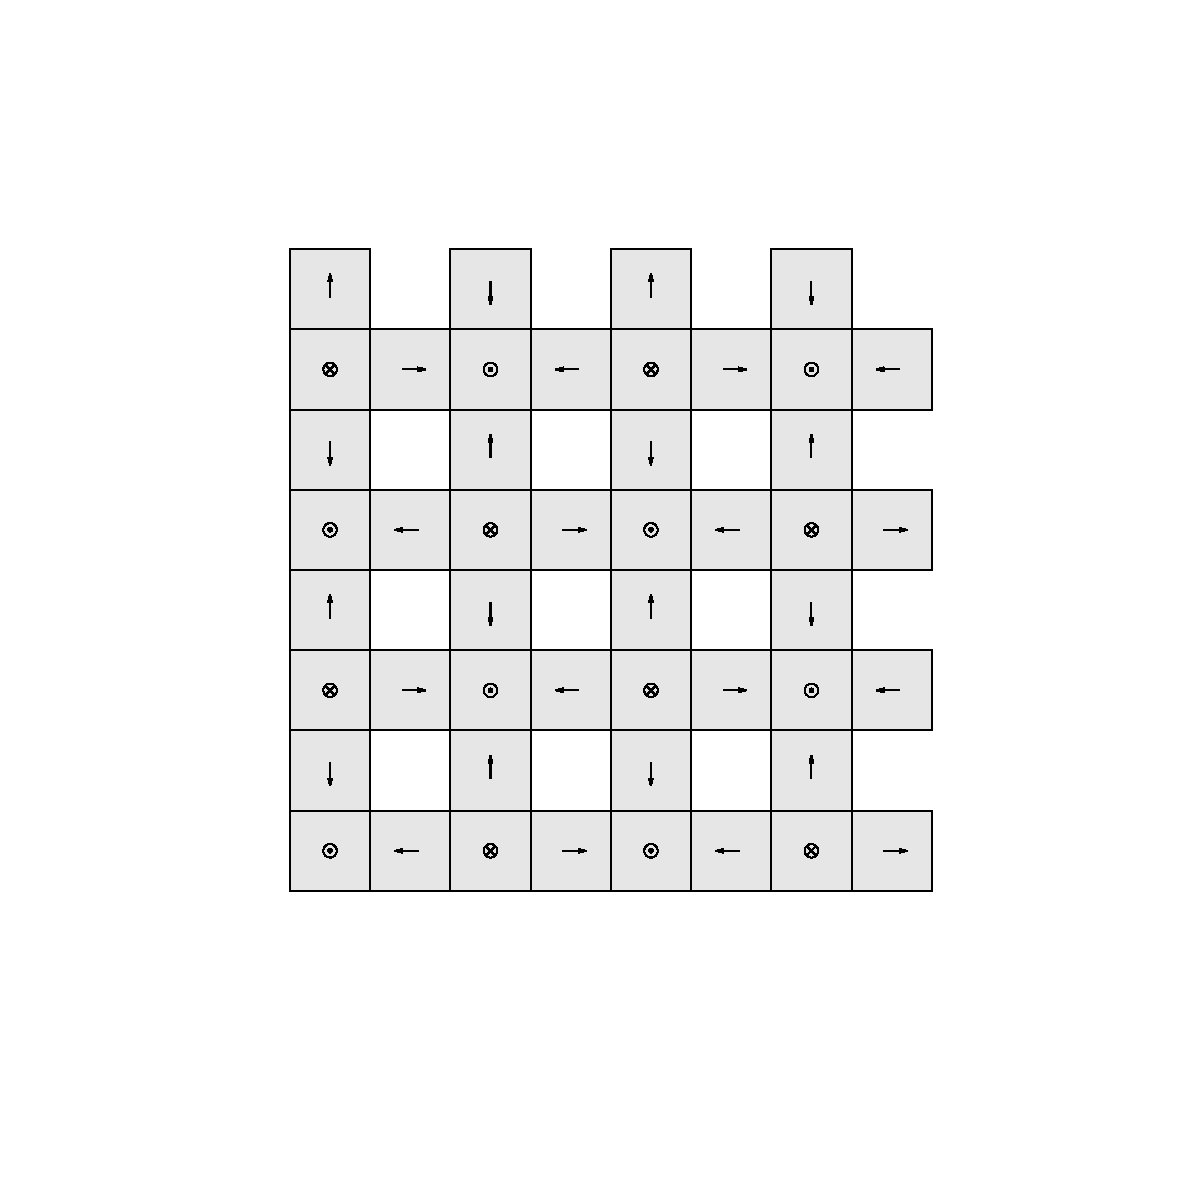
\includegraphics[width=\linewidth]{images/cuboidPlanarArraypdf.pdf}
        \vspace{-30mm}\subcaption{}
    \end{subfigure} \\
    \begin{subfigure}{\linewidth}
        \centering
        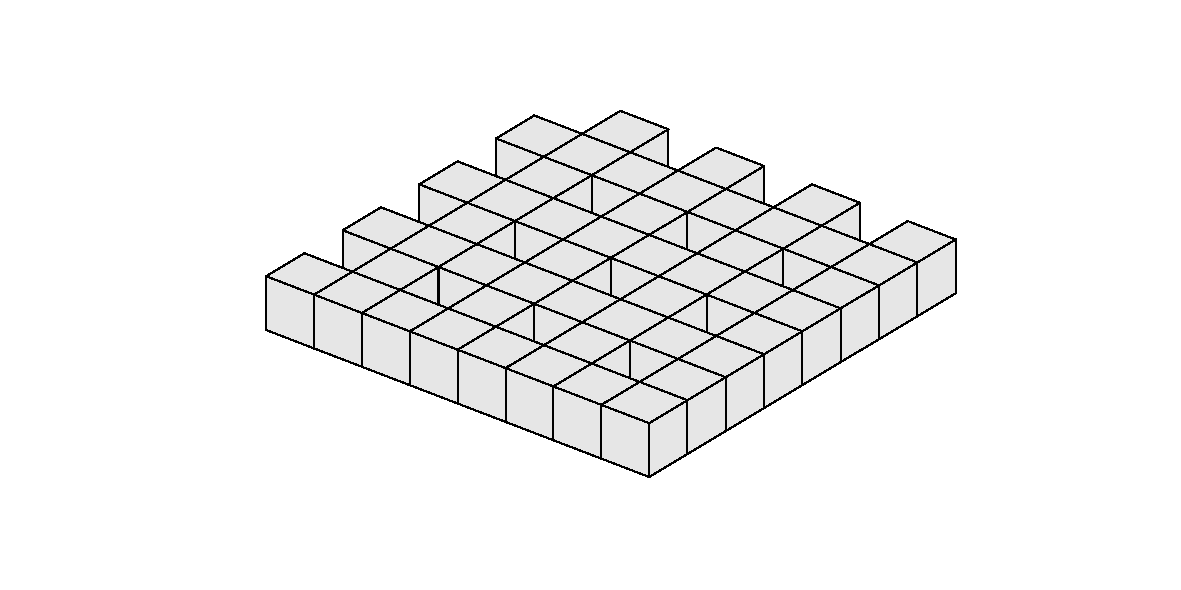
\includegraphics[width=\linewidth]{images/cuboidPlanarArrayAngledpdf.pdf}
        \vspace{-10mm}\subcaption{}
    \end{subfigure}
    \caption{Top view (a) and trimetric view (b) of a planar Halbach array created using cube permanent magnets. These are simple to produce, as only one configuration of magnet is required.}
    \label{fig:planarHalbachArray}
\end{figure}
However, to achieve the Halbach magnetisation pattern in two dimensions, some parts of the array must be empty, leading to unused space in the array. Many authors have attempted to optimise the planar array by modifying the relative size of the magnets, potentially reducing the unused space (Figure \ref{fig:planarHalbachArrayModifiedPoles}). Often, the magnets with magnetisations parallel to the plane are made smaller, while those with magnetisations orthogonal to the plane are made larger. In this way, the empty space in the array is reduced, while maintaining the Halbach magnetisation pattern.
\begin{figure}
    \centering
    \begin{subfigure}{\linewidth}
        \centering
        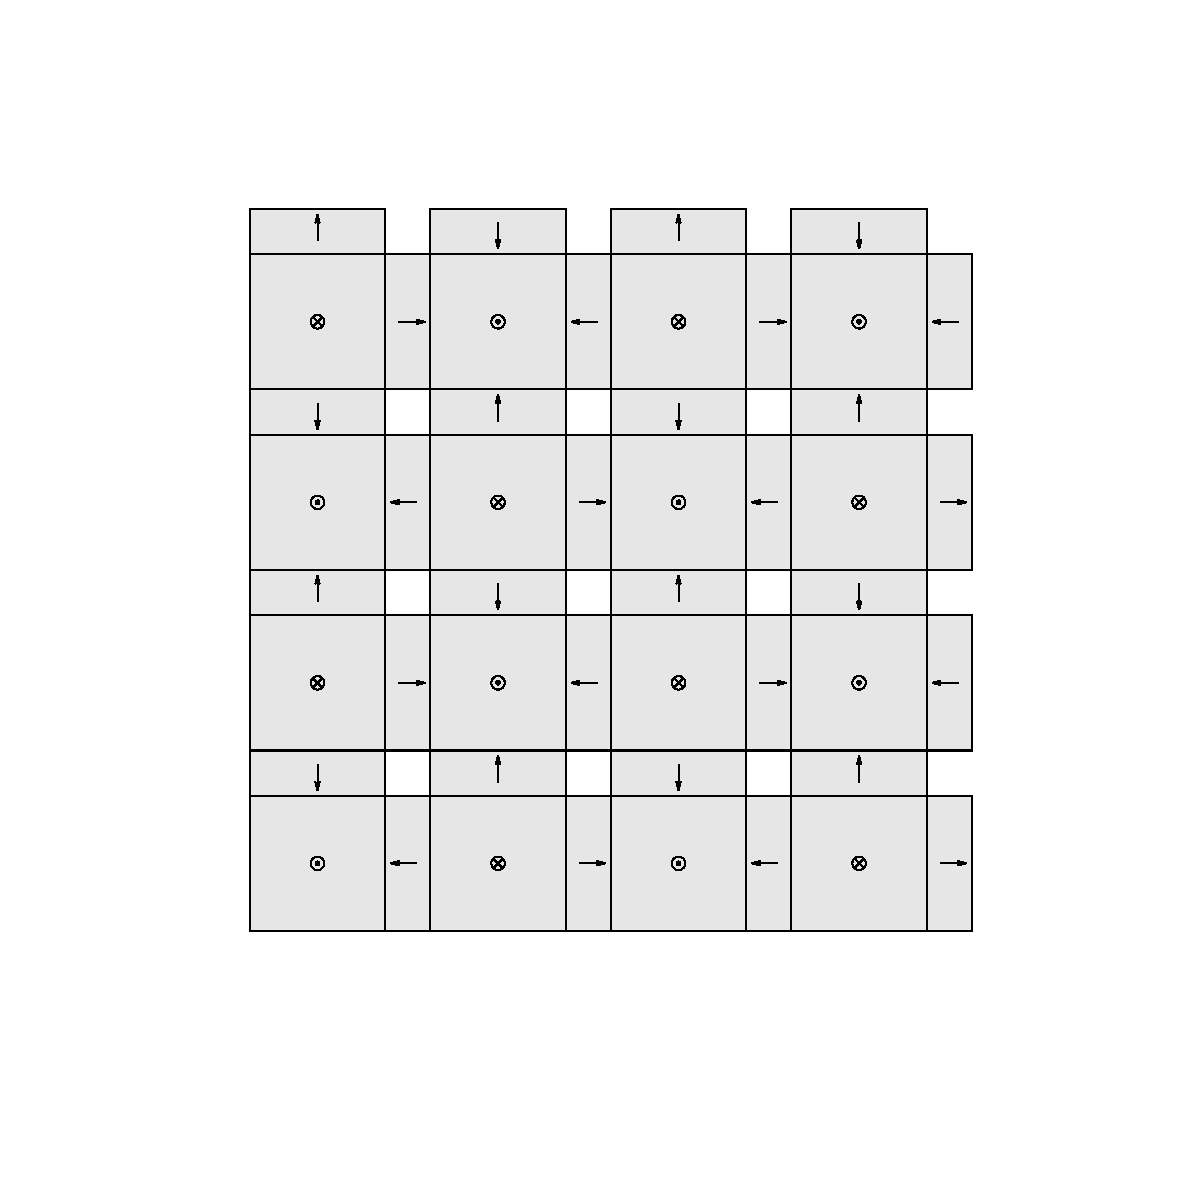
\includegraphics[width=\linewidth]{images/cuboidPlanarArrayReducedSpacepdf.pdf}
        \vspace{-25mm}\subcaption{}
    \end{subfigure} \\
    \begin{subfigure}{\linewidth}
        \centering
        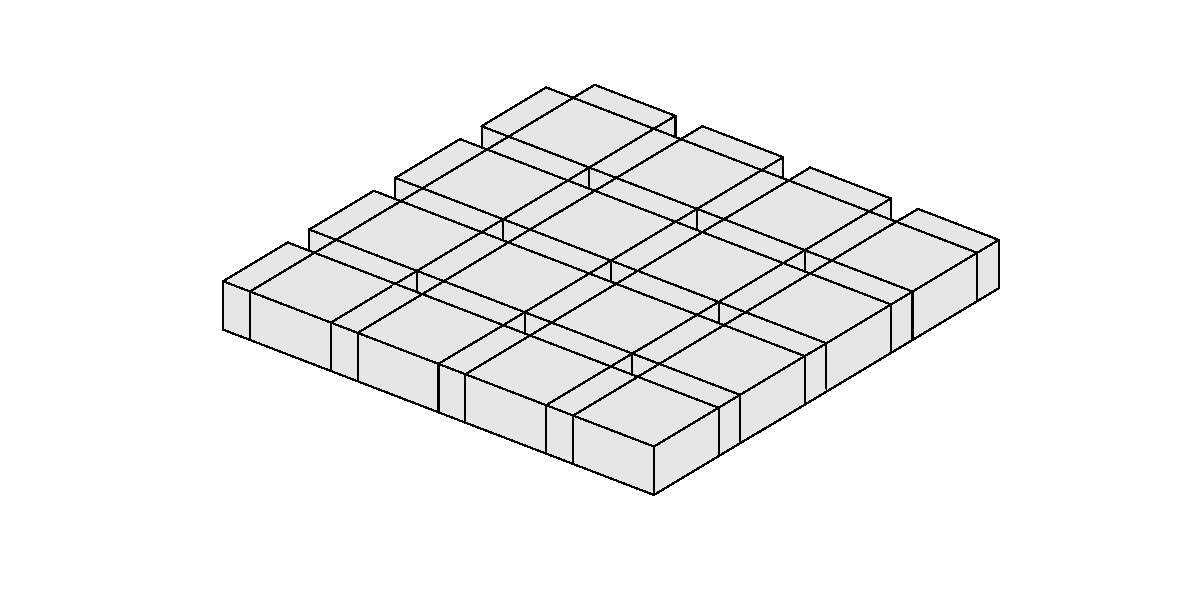
\includegraphics[width=\linewidth]{images/cuboidPlanarArrayReducedSpaceAngledpdf.pdf}
        \vspace{-10mm}\subcaption{}
    \end{subfigure}
    \caption{Top view (a) and trimetric view (b) of a planar Halbach array in which the magnets with magnetisations orthogonal to the array are made larger, thus reducing the empty space in the array.}
    \label{fig:planarHalbachArrayModifiedPoles}
\end{figure}
\begin{figure}
    \centering
    \begin{subfigure}{\linewidth}
        \centering
        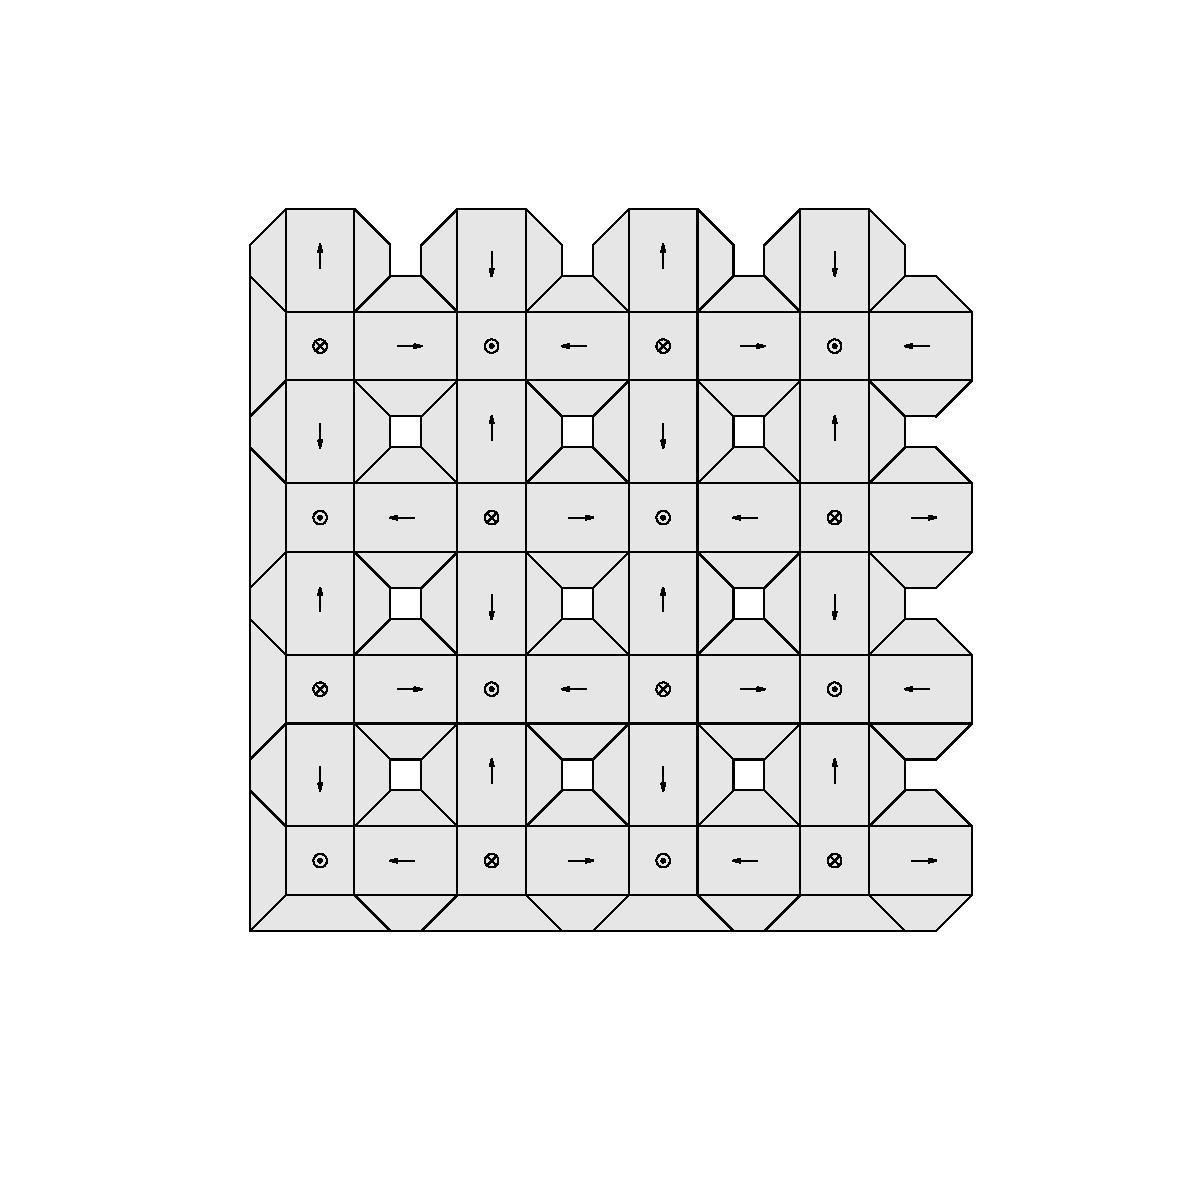
\includegraphics[width=\linewidth]{images/frustumPlanarArraypdf.pdf}
        \vspace{-25mm}\subcaption{}
    \end{subfigure} \\
    \begin{subfigure}{\linewidth}
        \centering
        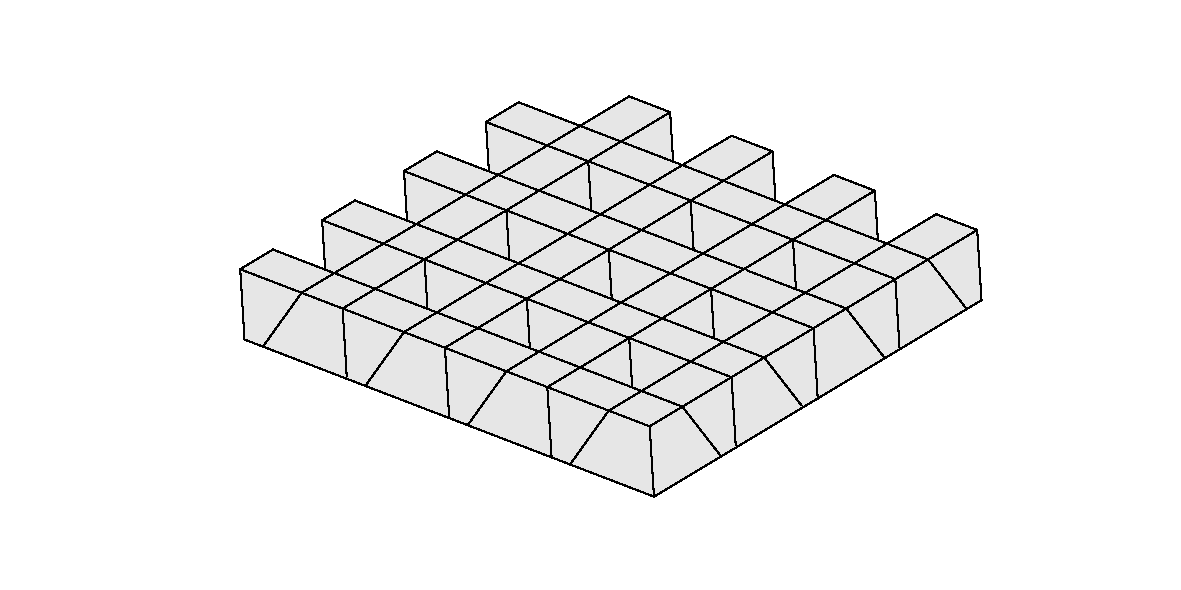
\includegraphics[width=\linewidth]{images/frustumPlanarArrayAngledpdf.pdf}
        \vspace{-10mm}\subcaption{}
    \end{subfigure}
    %\vspace{10cm}
    \caption{Top view (a) and trimetric view (b) of a planar Halbach array using pyramid and tetrahedral frustum magnets. This is the planar equivalent of the linear Halbach array with trapezial prismatic magnets shown in Figure \ref{fig:trapezoidalPrismaticHalbach}.}
    \label{fig:planarHalbachArrayPolyhedral}
\end{figure}

Further variations on planar Halbach geometry have been done, such as increasing the number of magnets for each repeating unit of the array. This leads to a more desirable field pattern with a larger field component orthogonal to the array while reducing the higher order harmonics of the field produced \cite{Min2010}. In addition, some authors have experimented with triangular prismatic magnets \cite{Cho2001,Cho2002} and frustum permanent magnets (Figure \ref{fig:planarHalbachArrayPolyhedral}) \cite{Peng2013,Janssen2009,Janssen2010a}, finding more desirable fields by varying and optimising magnet geometry.

\subsection{Permeability}
The effect of permeability leads to considerable difficulty in modelling permanent magnets. In essence, when a permanent magnet is exposed to a magnetic field, including its own, the magnetisation vector field is altered, with the effect being more significant for larger permeability. This is depicted in Figure \ref{fig:permeabilityOnMagnet}, with the top magnet being ideal, but the remanence magnetisation \(\mathbf{B}_r\) of the bottom becoming weaker due to its permeability, and some of the `magnetic charge' leaking to the sides of the magnet. The alteration of the magnetisation vector field leads to an altered field through the magnet, leading to further alteration of the magnetic vector field, and so on. In addition, the field through a magnet is not spatially constant; the field at one point inside a magnet is usually different from the field at another point. Thus, the magnetisation vector field is spatially varying, considerably increasing the modelling difficulty.
\begin{figure}
    \centering
    \begin{subfigure}{\textwidth}
        \centering
        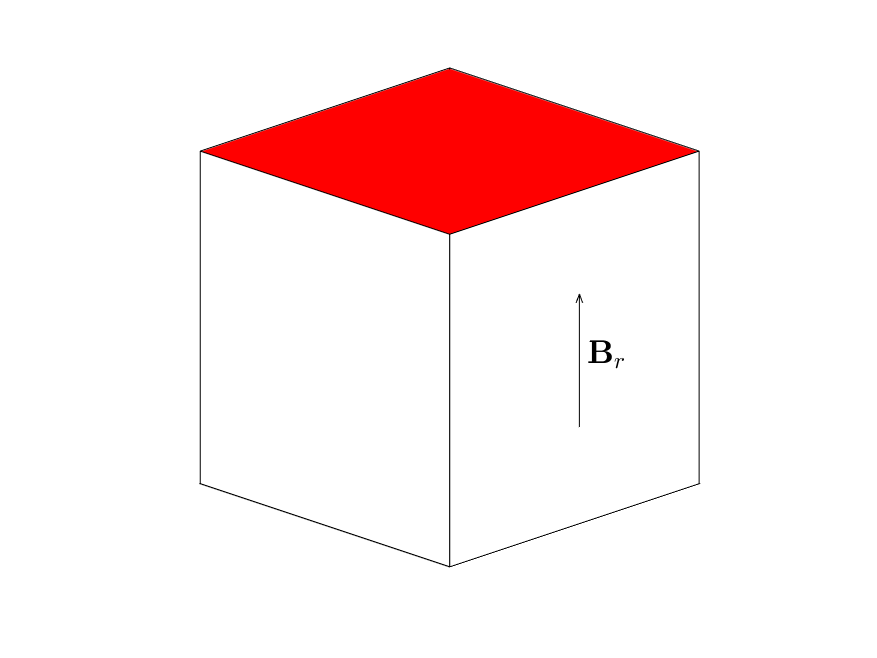
\includegraphics[width=0.65\linewidth]{p4/p4FIG1a}
        \caption{}\label{fig:introSingleMagnetIdealised}
    \end{subfigure}
    \begin{subfigure}{\textwidth}
        \centering
        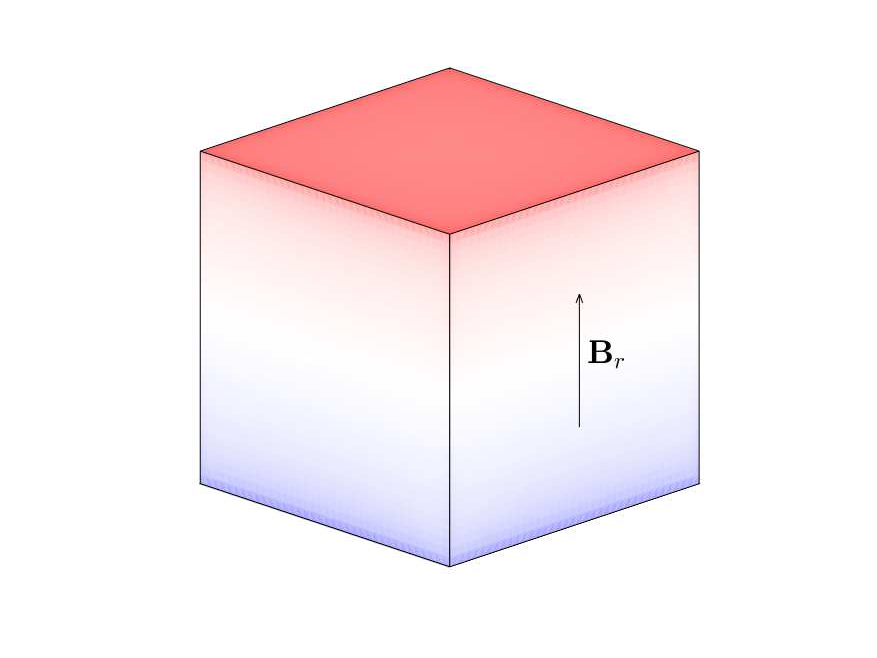
\includegraphics[width=0.65\linewidth]{p4/p4FIG1b}
        \caption{}\label{fig:introSingleMagnetNonideal}
    \end{subfigure}
    \caption{An ideal permanent magnet with relative permeability \(\mu_r = 1\) (\subref{fig:introSingleMagnetIdealised}), with the equivalent magnet but with permeability \(\mu_r = 3\) (\subref{fig:introSingleMagnetNonideal}). In the latter case, the surface charge is `leaking' onto the sides of the magnet under its own self-field, resulting in a weaker magnet overall.}
    \label{fig:permeabilityOnMagnet}
\end{figure}

Permanent magnets often have low permeabilities, with common values presented in Table \ref{tab:permeabilityClassificationTable}. Commonly used modern rare-earth neodymium magnets, for example, have a relative permeability of \(\mu_r \approx 1.05\). Therefore, the effect of permeability is small. Due to this, most research models permanent magnets with a relative permeability of unity, neglecting the effect of permeability as highlighted earlier in Section \ref{sec:geometrySolutions}. However, \textcite{Rovers2013} showed a nontrivial error when neglecting the permeability. Specifically, they modelled a cuboidal magnet with relative permeability \(\mu_r = 1.1\) and found an error of approximately 4\% in the magnetic field strength. They were able to mitigate this error by using the method of images to find an equivalent magnetisation vector. Similarly, \textcite{Kremers2013} found an expression for the equivalent magnetisation vector using the properties of permeability across the boundary of a magnet. It should be noted, however, that these studies do not consider spatially-varying magnetisation.

Other methods to model magnetic permeability involve subdividing a magnetic specimen into multiple surface or volume elements. For instance, \textcite{Forbes2021} subdivides a ring magnet into ring sector volumes, each being magnetically linear. This allows the modelling of nonlinear materials near saturation. Similarly, \textcite{Zhang2021} subdivides a cuboidal magnet into a large number of smaller cuboidal magnets and uses the magnetic surface charge method on each to calculate the total field. In contrast, \textcite{Casteren2014} subdivides the surface of a cuboidal magnet into small surface elements, each with their own surface charge density which is adjusted based on the field. However, each of these three methods requires iteration, since a change in the magnetisation vector or surface charge density changes the field, which requires further adjustment of the magnetisation vector or surface charge density, and so on, which can lead to considerable computation time.

\subsection{Literature summary}
Three-dimensional magnetostatic modelling of permanent magnets was first accomplished less than forty years ago. While much work has been done since, there are still many open problems, such as the force and torque between cuboidal magnets under general rotations, or the most optimal configuration for magnets in an array. Of particular interest to this thesis is the magnetic fields produced by polyhedral permanent magnets. While studies have derived equations for these fields, these equations are often complicated and computationally expensive, leading to slow force and torque calculations. Similarly, the magnetostatic modelling of permeability has been studied over the last decade, and solutions have been presented, but with a high computational cost. Therefore, this thesis aims to target the magnetostatic modelling of the magnetic fields, forces, and torques associated with permeable polyhedral permanent magnets.

\section{Thesis aims and scope}
Much of the current magnetic modelling literature is highly geometry-specific and requires ideal conditions. For example, the work by \textcite{Akoun1984} requires two magnets to be cuboidal with constant, uniform magnetisation vectors in the same direction, with both magnets having a relative permeability of unity. While other research is often more general than this, most is still rather specific. This thesis aims to further generalise magnetic modelling techniques by reducing the reliance on both magnet geometry and magnet permeability in a computationally efficient methodology.

The first primary objective of this thesis is to find new expressions for the magnetic field produced by general polyhedral permanent magnets, and to apply these to estimate forces and torques between these magnets. This is done by solving the magnetostatic charge model for generalised polyhedral magnets with unity relative permeability. The methodologies found are applicable to any magnet composed of flat faces, and magnets with curved faces may be approximated with polyhedra and the methodologies applied. The methodologies are also used to analyse planar arrays of magnets for use in a planar actuator.

The second objective of this thesis is to derive a method to model magnetically linear permeable materials of polyhedral geometry. This is based on the theory of permeability and uses the methods from the first objective to estimate the magnetic fields, forces, and torques produced by magnetically linear polyhedral magnetic materials.

Both objectives are undertaken with computation efficiency in mind. Vectorised code is used where possible, and mathematical expressions are simplified to avoid unnecessary computations. The equations and methodologies are implemented in interpreted MATLAB code. While compiled C++ code may be faster, MATLAB code provides far more flexibility and rapid prototyping of code due to the interpretive nature. While parallelised code can dramatically increase computation speed of large problems, the overhead associated with parallelisation may hurt the computation of small problems. As such, most code is non-parallelised, with the exception of the large optimisation problem in Chapter \ref{chap:paper3}.

In summary, achieving the main aims and objectives in this thesis will allow fast and accurate modelling of permanent magnets and other linear magnetic materials.

\section{Thesis format}
This thesis is presented in a \textit{Thesis by publication} format, with three articles (forming Chapters \ref{chap:paper1} to \ref{chap:paper3}) published, and one article (forming Chapter \ref{chap:paper4}) submitted. All articles have been submitted to high ranking journals in the magnetic modelling area of research.

\section{Thesis outline}
This thesis begins with a brief historical overview of the development of electromagnetism as a science, commencing with the first recordings of magnetism, and concluding with the discovery of quantum mechanics and electron spin.

Chapter \ref{chap:introduction} follows, detailing the mathematical background of magnetism and giving a review of current literature on magnetic modelling. This chapter outlines the current gaps in knowledge of the magnetic science, and summarises the main purpose of this thesis.

The substantive work of the thesis begins in Chapter \ref{chap:paper1}, which details a methodology to evaluate the magnetic field produced by a polyhedral magnet and estimate the force and torque between two polyhedral magnets. While this method is effective when calculating the magnetic field at a single point, it becomes less efficient when evaluating the field at many points. Therefore, a new method was found, presented in Chapter \ref{chap:paper2}, which presents solved field equations which are considerably more effective when calculating the field at many points. This is useful for force and torque evaluation, since a numeric surface integral requires the field evaluated at each surface element, with a larger number of field evaluations leading to a more accurate force and torque result.

Chapter \ref{chap:paper3} presents a case study on planar Halbach arrays by using the methodology described in Chapter \ref{chap:paper2}. This explores using pyramid and tetrahedral frustum permanent magnets rather than the more traditional cuboidal magnets in a planar array.

The work presented in Chapters \ref{chap:paper1} to \ref{chap:paper3} require a relative permeability of unity, limiting their use case in real magnetic systems. To alleviate this limitation, Chapter \ref{chap:paper4} investigates magnetic permeability and details a method for modelling permeable permanent magnets. This method attempts to alleviate the requirement for iteration by calculating the magnetic field only once and performing a matrix inversion. This considerably reduces computation time at the cost of computational memory.

Finaly, the thesis is concluded in Chapter \ref{chap:conclusion}, which summarises the thesis as a whole and outlines potential future work to follow this thesis.
\newpage
\section*{References}
\addcontentsline{toc}{section}{\protect\numberline{}References}
\printbibliography[heading=none]